\chapter{State of the Art}
\label{chap:SOTA}

This chapter examines the State of the Art, in the context of this dissertation. Section \ref{sota:5gecosystem} begins by performing an overview of the current state of the \acs{5G} ecosystem, introducing foundational concepts such as network slicing, virtualization, and the integration of \acs{SDN} and \acs{NFV}. Section \ref{sota:slicing} discusses network slicing, further detailing its concept and the lifecycle management of a network slice instance. It also presents two network slice managers and its capabilities: (i) the Katana Slice Manager~\cite{KatanaSliceManagerWiki} and (ii) \acs{ITAv}'s Slice Manager~\cite{ITAvSliceManager}. Then, Section \ref{sota:nfv} describes the concept of \acf{NFV} and the \acf{NFV-MANO} framework.

Afterwards, Section \ref{sota:sba} describes the \acs{5G} \acf{SBA} and its constituent network functions. The network exposure capabilities specified by \acs{3GPP} are also discussed, along with an analysis of the various available \acf{NEF} implementations used throughout the literature. Section \ref{sota:networkapplications} defines the concept of network applications, focusing on services and use cases that benefit from \acs{5G} capabilities. These applications rely on key telco standardization initiatives, highlighted in Section \ref{sota:telcoinitiatives}.

Subsequently, Section \ref{sota:bss-oss-mano} addresses the supporting and management systems that allow efficient operations and orchestration of modern networks, covering \acfp{BSS}, \acfp{OSS} and the benefits of integrating them with \acs{NFV-MANO} systems. Then, testbed implementations reported in the literature are analyzed, presenting the various components of the testbeds at the level of the \acs{5G} Core, \acs{5G} \acs{RAN} and network exposure interfaces, as discussed in Section \ref{sec:testbeds:main}.

Lastly, Section \ref{sec:testingandvalidation} focuses on the testing and validation procedures implemented to evaluate network-aware applications and scenarios, emphasizing the various methodologies, metrics and pipelines used to verify compliance with functional and non-functional requirements. 


\section{The 5G Ecosystem} \label{sota:5gecosystem}

% verify rough cites
% should I cite multiple here? because roadTowards6G cites imtVision5G but the definitios are more defined on the imtVision2015
The introduction of the \acf{5G}, marks a paradigm shift in mobile communications, establishing a ubiquitous connectivity platform~\cite{tech-leadership-and-5g-patent-portfolios} and contributing to the promise of a fully connected society. \acs{5G} represents more than just an incremental performance improvement over its predecessors with increased speeds and lower latencies in data transmissions, connecting people, machines and objects and accelerating digitalization in a variety of sectors. In fact, the success of \ac{IoT} and its wide variety of services and applications is supported, in part, by the development and deployment of \acs{5G}, and eventually of \acs{6G}~\cite{future-of-5g-beyond}. In order to encompass this diverse set of usage scenarios and applications, \acs{5G} was designed to support three classes of services~\citep{imtVision2015, roadTowards6G}:
\begin{itemize}
    \item \textbf{\ac{eMBB}:} addresses human-centric use cases for access to multi-media content, services and data. This usage scenario requires delivering enhanced data rates within high user density hostspot environments, where high traffic capacity is needed, and wide-area coverage scenarios that demand seamless coverage and high mobility. Compliance with these requirements fosters new applications over smart devices (smartphones, tablets, and wearable electronics), such as high-definition video streaming in densely populated urban hotspots, as well as \ac{AR} scenarios;
    \item \textbf{\ac{URLLC}:} caters safety and mission-critical services with stringent requirements on reliability, latency and availability. This includes applications such as autonomous vehicles, Smart Energy Grids and Industry 4.0;
    \item \textbf{\ac{mMTC}:} supports dense connectivity of a very large number of low-cost, long-battery-life \ac{IoT} devices typically transmitting a relatively low volume of non-delay-sensitive data at low data rates, for example, sensors.
\end{itemize}

Given this wide diversity of traffic profiles, each demanding distinct performance characteristics, network slicing is introduced to cator to the heterogeneous \ac{QoS} requirements across the different service classes. Network slicing allows the physical network to be partitioned (sliced) into multiple isolated logical networks, each tailored to different types of services with distinct characteristics and requirements. This approach enables the provision of customized reliable services using limited network resources, thereby reducing the \ac{CAPEX} and \ac{OPEX} of \ac{5G} networks~\cite{networkSlicingBased5GFutureMobileNetworks}. By leveraging network slicing, operators can create different levels of services, allowing customized operations for different industry verticals~\cite{NetworkSlicingUseCasesGSMA}. Enterprise verticals operate within distinct vertical domains, defined as specific industries, sectors or groups of enterprises in which similar products or services are developed, produced and provided through applications, commonly referred to as vertical applications~\cite{SEAL5GVerticals}.

The implementation of network slicing is supported by virtualization technologies, which abstract software functions from the physical hardware, eliminating the need for dedicated equipment. This abstraction contrasts with the traditional approach of monolithic and proprietary hardware appliances based on specific implementations that would require significant modifications and an increased cost to introduce new network services and accommodate new service requirements~\cite{networkSlicingOverview}.

More specifically, one of the key enabling technologies of \ac{5G} network slicing is \ac{NFV}. \ac{NFV} addresses the virtualization of network functions, such as firewalls, as \acp{VNF}, on top of commodity hardware devices, breaking the traditional vendor approach of tightly coupled software and hardware offerings. By decoupling the software from the hardware platform both can evolve independently from each other, providing a greater flexibility to deploy new innovative software services (network functions) using the same hardware platform~\cite{slicingUsingSdnNfvTaxonomy}. 

With software-based \ac{NFV} solutions, some of the \acp{NF} can be placed at the \ac{SP}'s shared infrastructure. Therefore, modifying functions for all or a subset of customers becomes much more manageable since changes can be performed centrally at the \ac{SP}'s infrastructure rather than at the customer premises. Additionally, \ac{NFV} offers \acp{SP} the ability to (i) dynamically scale and provision tailored network services based on customer demand, (ii) reduce both \ac{CAPEX} and \ac{OPEX} on network infrastructure and (iii) shorten the time-to-market for new network services~\cite{slicingUsingSdnNfvTaxonomy}.

% this is achieved through a centralized component -> can I infer this from the image?
\ac{SDN} plays a complementary role in network slicing, operating alongside \ac{NFV} to achieve softwarization and virtualization of the network infrastructure and resources, respectively. \ac{SDN} simplifies network management, introducing network programmability and open network access by decoupling the control plane from the data plane and logically centralizing network intelligence~\cite{NetworkSlicingSoftwarizationSurvey}. This is achieved through a centralized \ac{SDN} controller over a virtualized control plane that intelligently manages network functions, bridging the gap between service provisioning and network management. In the context of network slicing, the \ac{SDN} controller dynamically manages slices, enforcing network slice policies and resource orchestration. Combined with \acs{NFV}, both provide programmable control and management of network resources, enabling efficient network slicing~\cite{slicingUsingSdnNfvTaxonomy}


\hide{

3-how-disruptive-is-5g -> introduction of verticals and use cases

lacks citing all features from the sensors paper 

SAY THIS SOMEWHERE

- Providing a virtualized end-to-
end environment that can be opened to third
parties is one of the key features that differentiates
network slicing from network sharing.

- Network Slicing as a service (5g-network-slicing-using-SDN-and-NFV)

\later{check citations of systematic reviews and see if they are from the systematic review or from a specific source mentioned in the systematic review}

\later{ONF for network slicing}

\later{This way, the network control becomes directly programmable using standardized \aclp{SBI}  ~\cite{slicingUsingSdnNfvTaxonomy} defining communication between forwarding devices in the data plane and the control plane.}

- Supported by network slicing, network resources can be dynamically and efficiently allocated to logical network slices according to the corresponding QoS demands.

}




\section{Network Slicing} \label{sota:slicing}

\later{add NSaaS somewhere}

\acs{5G} networks have been regarded by the industry and academia as a critical advancement in the support of next generation vertical applications, tailored to different service requirements and characteristics. This capability is accomplished through network slicing, which allows the creation of \acs{E2E} logical networks (network slices) on a common underlying infrastructure. Network slices are  self-contained, mutually isolated, independently managed and controllable to support programmable multi-service and multi-tenancy environments on a shared infrastructure~\cite{slicingUsingSdnNfvTaxonomy}.

Network Slices support a variety of services, expanding the traditional \acs{5G} service types introduced earlier (\acs{eMBB}, \acs{URLLC} and \acs{mMTC}) into a standardized set of \acf{SST} values, with \acs{SST} values 1,2,3,4,5 and 6 corresponding to \acs{eMBB}, \acs{URLLC}, \acs{mMTC}, \acf{V2X}, \acf{HMTC} and \acf{HDLLC}, respectively~\cite{ETSI_TS_123_501_V16_9_0}. 

\subsection{Network Slice Design \& Instance Lifecycle} \label{sec:slice:lifecycle}

The \acf{GST} by \acs{GSMA} provides a standardized list of attributes that characterize the different types of network slices and, consequently, of services. However, it is designed to be generic, not tied to any specific type of network slice or agreement between a \acf{NSC} and a \acf{NSP}. The \acs{GST} serves as the baseline for creating \acfp{NEST}, with specific values being assigned to the \acs{GST} to express a given set of requirements and support a network slice customer use case~\cite{GSMA_GST}. 

\acsp{NSP} can build their network slice product offerings based on \acsp{NEST}, encapsulating the concrete performance characteristics offered to the customer, which facilitates the establishment of \acfp{SLA} between operators and verticals and fosters interoperability. More specifically, \acsp{NEST} are the foundation for the \acs{NSP} deployment of a network slice, representing the initial step in the \acf{NSI} lifecycle, i.e. network slice preparation~\cite{GSMA_GST}.

\begin{figure}[H]
    \centering
    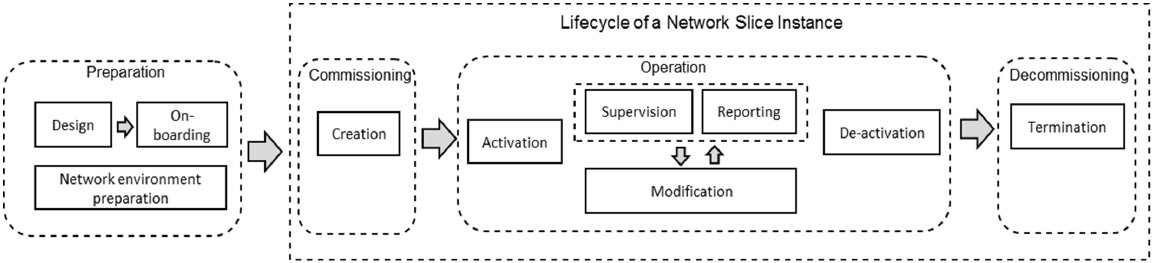
\includegraphics[width=1\linewidth]{figs/NSI_lifecycle.png}
    \caption{\acs{NSI} Lifecycle~\cite{ETSI_MANAGEMENT_ORCHESTRATION_CONCEPTS}}
    \label{fig:slicing:NSI_lifecycle}
\end{figure}

The \acs{NSI} encompasses the full set of Network Function instances and the required resources (e.g. compute, storage and networking resources) of a deployed Network Slice~\cite{ETSI_TS_123_501_V16_9_0} and its corresponding lifecycle is composed by the following phases highlighted in Figure \ref{fig:slicing:NSI_lifecycle}~\cite{ETSI_MANAGEMENT_ORCHESTRATION_PROVISIONING,ETSI_MANAGEMENT_ORCHESTRATION_CONCEPTS}:

\begin{itemize}
    \item \textbf{Preparation:} At this stage, the \acs{NSI} does not yet exist. The \acs{NEST} is created, verified, and onboarded during this phase. It also includes, apart from network slice design, the on-boarding and evaluation of the network functions and all necessary preparations (e.g. network preparations) required before the creation of a \acs{NSI};

    \item \textbf{Commissioning:} The \acs{NSI} is created, which involves allocating and configuring all required resources to satisfy the network slice requirements;
    
    \item \textbf{Operation:} This phase includes the activation, supervision and reporting (related to performance, such as \acs{KPI} monitoring), resource capacity planning, modification and deactivation. The first activates the \acs{NSI}, making it ready to provide communication services, whereas the latter does the opposite. Resource capacity planning involves any actions that calculate resource usage based on \acs{NSI} provisioning and performance monitoring, deriving modification polices as a result of the calculation. \acs{NSI} Modification may be triggered by receiving new network slice requirements or as the result of supervision/reporting and it includes the creation or modification of the \acs{NSI} constituents. Capacity or topology changes correspond to examples of a \acs{NSI} modification;
    
    \item \textbf{Decommissioning:} Encompasses the decomissioning of the required non-shared constituents and the removal of the \acs{NSI} configuration from the shared constituents, after which the \acs{NSI} is terminated and ceases to exist.

\end{itemize}


\subsection{Network Slice Management Functions}

For the purpose of \acs{NSI} management, the concept of a \acf{NSS} is introduced. As outlined in Figure \ref{fig:slicing:class:diagram}, a \acs{NSS} represents a group of network functions (physical and/or virtualized) and their corresponding resources that form part or all of the constituents of a network slice. A \acs{NSS} may be shared between multiple other network slices or subnets and contain instances of \acf{CN} and/or \acf{AN} network functions. Additionally, it may also specify the \acf{TN} requirements necessary to support connectivity between the \acs{CN} and the \acs{AN} network functions within the network slice subnet, covering \acs{TN} topology requirements and individual \acs{TN} links' \acs{QoS} attributes requirements~\cite{ETSI_MANAGEMENT_ORCHESTRATION_CONCEPTS}.

The instantiation of a \acs{NSS} results in a \acf{NSSI}. Similarly, an \acs{NSI} may be composed of one or more \acsp{NSSI} that abide by the same constraints defined for the \acs{NSS} throughout this paragraph. For instance, instantiating an \acs{NSI} with \acs{RAN} and \acs{CN} components may entail defining each domain's component as a separate \acs{NSSI}, potentially shared across multiple \acsp{NSI}~\cite{3GPP-28.801}. Both these constructs must therefore be managed and coordinated correctly to ensure the correct operation of a network slice. 

\begin{figure}[H]
    \centering
    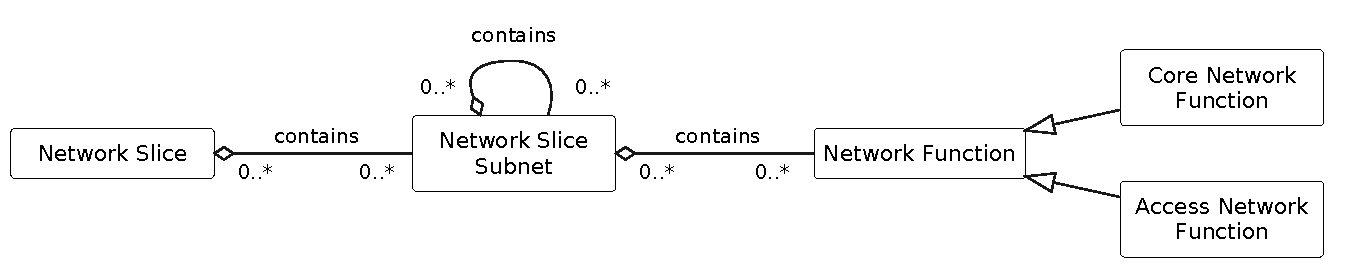
\includegraphics[width=1\linewidth]{figs/plantuml/network-slice-class-diagram.pdf}
    \caption{Network Slice Information Model~\cite{3GPP-28.801}}
    \label{fig:slicing:class:diagram}
\end{figure}

This section identifies three management functions involved in the management and orchestration of network slicing and, consequently, in the support of communication services: the \acf{CSMF}, the \acf{NSMF} and the \acf{NSSMF}. These management functions are organized in a hierarchical structure, where each function delegates part of the related procedures to the next function immediately after it, as showcased in Figure \ref{fig:slicing:management_functions}.

\begin{figure}[H]
    \centering
    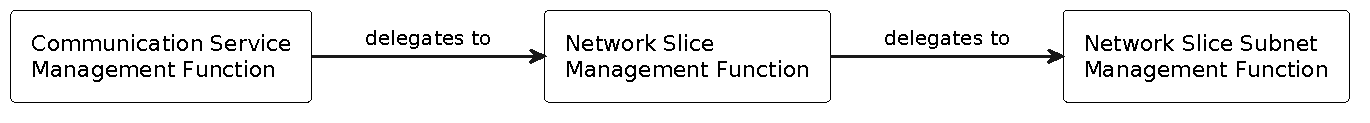
\includegraphics[width=1\linewidth]{figs/plantuml/network-slice-mgmnt-func.pdf}
    \caption{Network Slicing Management Functions~\cite{3GPP-28.801}}
    \label{fig:slicing:management_functions}
\end{figure}

The \acs{CSMF} is responsible for managing the communication services offered by an operator, receiving the requirements requested by end-customers and translating them into concrete network slice requirements, such as network type, network capacity and \acs{QoS} requirements~\cite{3GPP-28.801}. This functionality is closely aligned with that of an \acs{OSS}/\acs{BSS}, which will be further discussed in Section \ref{sota:bss-oss-mano}. These requirements are then forwarded to the \acs{NSMF}, which handles the management of \acsp{NSI} based on the provided requirements. Lastly, the \acs{NSMF} converts the network slice requirements to network slice subnet requirements, which are subsequently delegated to the \acs{NSSMF} for managing and orchestrating \acsp{NSSI}~\cite{3GPP-28.801}.

The management of network slices using these management services must span across the various parts of the network, including both \acs{3GPP} managed network components, such as the \acs{CN} and \acs{AN}, as well as non-\acs{3GPP} components. With this goal, the \acs{3GPP} management system derives each domain's requirements from the customer's service requirements (for a given communication service) and forwards them to the corresponding domain management systems, coordinating the exchange of data between them. For components outside the \acs{3GPP} domain, such as the \acs{TN}, this implies coordinating with the corresponding external management systems to communicate the network slice requirements~\cite{ETSI_MANAGEMENT_ORCHESTRATION_CONCEPTS}.

This is especially relevant, not only in the context of the \acs{TN}, but also considering the inherent virtualization nature of network slicing. When an operator wants to create a network slice, i.e. a \acs{NSI} that includes virtualized network functions, the \acs{NSSMF} should, per request from the \acs{NSMF}, create the needed \acsp{NSSI}, according to the network slice requirements. This involves coordinating with an external management system, namely the \acs{NFV-MANO}, to instantiate and configure all \acsp{VNF} and \acsp{NS}, scaling them as needed for the operations of the \acs{NSI}, while accounting for the fact that these resources may be shared by multiple \acsp{NSSI}. Only after coordinating with the \acs{NFV-MANO}, and performing the necessary application level configurations to the \acsp{NF} allocated to the \acs{NSSI}, the \acs{NSMF} can proceed with the activation of the \acs{NSI}~\cite{3GPP-28.801}.

\subsection{Network Slice Managers}

A Slice Manager is a software system that allows the orchestration and lifecycle management of network slices. The following section presents an overview of two slice managers: the Katana Slice Manager and \acs{ITAv}'s Slice Manager.

\subsubsection{Katana Slice Manager}

Katana is a slice manager solution developed as a part of the 5GENESIS project~\cite{KatanaSliceManagerGenesis}. Through its \acf{NBI}, it receives the \acs{NEST} for creating the network slices, providing an \acs{API} for managing and monitoring them. The \acs{NEST} descriptor, specified in \acs{YAML} or \acs{JSON}, specifies the network slice characteristics and parameters, including \acs{NFV} components, \acs{QoS} monitoring level and Life-Cycle stages. Based on the onboarded \acs{NEST}, the slice manager maps the available data plane resources to the described slice requirements in order to create the requested slice. Additionally, the slice manager communicates with the components from the Management Layer through its \acs{SBI}, including the \acf{VIM}, \acf{NFVO}, \acf{EMS} and \acf{WIM}.

To accommodate multi domain testbed environments, it was developed as a standalone solution that interacts with other components of the \acf{MANO} layer via the defined interfaces (e.g. through SOL005 interface for \acf{OSM} \acf{NFVO}), as to allow the management of the network slice's lifecycle without extended \acs{MANO} functionality~\cite{KatanaSliceManagerGenesis}

\begin{figure}[H]
    \centering
    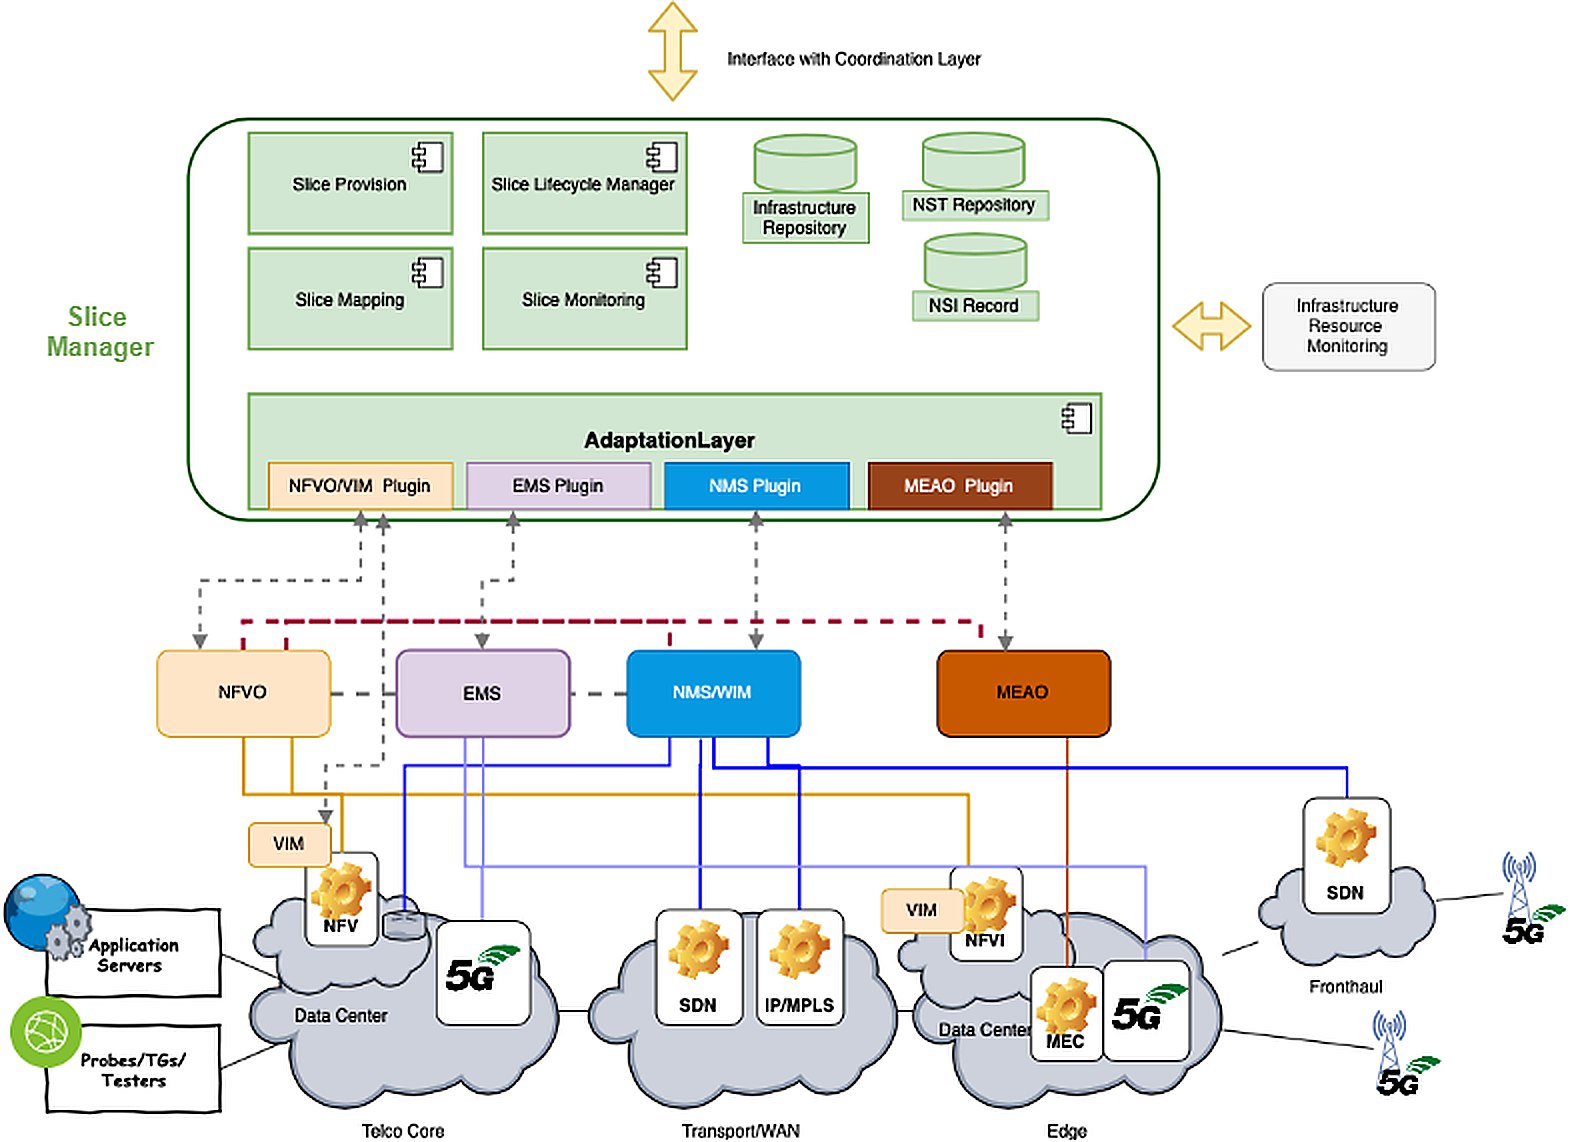
\includegraphics[width=0.95\linewidth]{figs/katana-architecture-upscaled.png}
    \caption{Katana Slice Manager Architecture~\cite{KatanaSliceManagerWiki}}
    \label{fig:katana:architecture}
\end{figure}


The Katana Slice Manager follows a highly modular architecture, implemented as a mesh of independent microservices, each running in a dedicated Docker container. Figure \ref{fig:katana:architecture} illustrates the architecture of the slice manager, highlighting its constituent modules and their interconnections, as described bellow~\cite{KatanaSliceManagerWiki}.

\customparagraph{North Bound Interface API}

The \acf{NBI} provides a set of \acs{REST} \acsp{API}, to be consumed by a component of the coordination layer, such as the Experiment Lifecycle Manager. It includes two submodules that consume these \acs{REST} \acsp{API}, allowing a user or admininstrator to interact with it: (i) a \acf{CLI} for Bash commands interaction via the terminal and a (ii) web \acf{GUI} that interacts with the Slicing Lifecycle Manager and repositories to create new slices. 

\customparagraph{Slicing Lifecycle Manager}

This module serves as the central component of the slice manager, responsible for managing the lifecycle of network slices through \acs{CRUD} operations. It handles requests from the \acs{NBI} \acsp{API} and executes the required actions to activate, modify or deactivate a network slice. Additionally, it receives status updates from the Slice Monitoring module regarding a given slice, coordinating with other components to trigger the appropriate processes in response to these changes. Lastly, it is also tasked with optimally selecting the infrastructure resources to be used for a new slice, according to the available resources and the slice requirements, during the slice creation phase.

\customparagraph{Slice Mapping}

The Slice Mapping component manages the slice mapping process, following the request for a new slice. It maps the \acs{GST} requests with a specific \acs{NEST} that is supported by the infrastructure.

\customparagraph{Slice Provisioning}

Receives requests from the Slicing Lifecycle Manager service to setup, configure or delete \acs{WAN} paths, isolated \acs{NFVI} tenant spaces and the related network services. It also manages the configuration of radio component parameters and the registration of the newly created slice into the Monitoring system. All of the aforementioned functionalities are achieved by utilizing plugins of the Adaptation Layer.

\customparagraph{Slice Monitoring}

This module is responsbile for monitoring the health and the status of every deployed slice. Similarly to the previous service, it relies on Adaptation Layer plugins to send status check messages to the \acs{MANO} components and report status changes to the Slicing Lifecycle Manager.

\customparagraph{Adaptation Layer}

The Adaptation Layer provides an abstraction layer over the underlying technology, allowing the slice manager to operate over any \acs{MANO} layer component without any modifications to its core functionality, given the correct plugin is installed. This module includes plugins for each of the slice manager's \acs{MANO} layer components, which are responsible for receiving and translating requests from the Slicing Lifecycle Manager into the corresponding component \acs{API}, and, consequently, processing the responses.


This architecture provides the baseline for the provisioning and lifecycle management of network slices. However, the Katana open source project has been inactive, with no updates since December 2022, rendering it unusable for this dissertation. It does not support more recent \acs{OSM} versions, with the latest compatible release being \acs{OSM} 8.


\subsubsection{ITAv Slice Manager}

\acf{ITAv} has its own proprietary implementation to automate the deployment and management of network slices in \acs{5G} networks~\cite{ITAvSliceManager}. The \acs{ITAv} Slice Manager is currently deployed on the 5GAIner testbed~\cite{5GAIner}, a commercial-grade \acs{5G SA} infrastructure also available at \acs{ITAv}. The solution enables the programmatic reconfiguration of the \acs{5G} network, provisioning slices tailored to meet the requirements of the three primary \acs{5G} services: \acs{eMBB}, \acs{URLLC} and \acs{mMTC}/\acs{MIoT}. The slices configured by the network slice manager preserve the network \acf{TRL}, being the produced
slices representative of a commercial-graded solution. Moreover, the slice manager also offers dynamic slicing capabilities, supporting the adaptation of the slice performance in real time without communication disruption.

The \acs{ITAv} Slice Manager is designed with a strong focus on adherence to established standards to ensure interoperability and seamless interaction with other software systems, as defined by \acs{3GPP}. In particular, it complies with the following specifications:

\begin{itemize}
    \item 3GPP TS 28.531 version 18.3.0~\cite{ITAv_3gpp_28531_v18_3_0}: outlines the essential Network Functions for a standardized network slice manager;
    
    \item 3GPP TR 28.824 version 18.1.0~\cite{ITAv_3gpp_28824_v18_0_1}: identifies the \acf{TMF} standards required for the Slice Manager, with adherence to TMF622\_ProductOrder~\cite{TMF622UserGuideV5} and TMF641\_ServiceOrder~\cite{TMF641UserGuideV411}, as defined in December 2023;

    \item 3GPP TS 28.541 version 18.4.1~\cite{ITAv_3gpp_28541_v18_4_1}: delineates the profiles associated with network slices (e.g. ServiceProfile, TOPSliceSubnetProfile);

    \item 3GPP TS 28.530 version 17.4.0~\cite{ITAv_3gpp_28530_v17_4_0}: presents the Network Slice Management Lifecycle.
\end{itemize}

According to the original work~\cite{ITAvSliceManager}, the \acs{ITAv} Slice Manager supports an extensive list of Slice Manager requirements identified throughout the literature: \ac{E2E} Slice Support, Slice Lifecycle Management, Network Configuration, Policy and \acs{QoS} Management for \acs{SLA} Enforcement, Dynamic Slicing, Custom Slices, Network Slice Monitoring, Location-based Slicing, Performance Assurance, Multiple Slice Management, Network Resource Monitoring, Slice Feasibility Evaluation, and Generic Network Support. Furthermore, the slice manager solution can be integrated with \acs{OSM} and \acf{OSL}, allowing adherence to an even more complete set of requirements with orchestration and \acf{OSS} capabilities~\cite{ITAvSliceManager}. The \acs{ITAv} Slice Manager represents a significantly more mature solution than the available alternatives.



\section{NFV} \label{sota:nfv}

As outlined in Section \ref{sota:5gecosystem}, the implementation of network slicing is supported by virtualization technologies, such as \acs{SDN} and \acs{NFV}, which have fundamentally transformed how networks are managed and deployed. With the growing adoption of \acs{SDN} and \acs{NFV} technologies, network functions are no longer tied to dedicated hardware instead being instantiated dynamically as software components in cloud environments. This allows operators, partners and even subscribers to create instances of their services and networks on demand~\cite{EricsonOSS}. 

This section examines the concept of \acs{NFV} and its realization through the \acf{NFV-MANO} framework. It provides an analysis of the \acs{NFV-MANO} architecture and its constituent functional blocks, detailing their respective roles and interactions in enabling the deployment and orchestration of virtualized network services.


\subsection{NFV-MANO Architectural Framework}

As previously stated, \acs{NFV} refers to the principle of separating network functions from the underlying running hardware using virtualization techniques. This approach results in \acfp{VNF}, software solutions that realize all or part of a \acf{NF} and can be deployed in the \acf{NFVI}~\cite{ETSI_GR_NFV_TERMINOLOGY_003_V1_9_1}. A \acf{NS} is then defined as the composition of one or more \acsp{NF} (\acsp{VNF} or \acsp{PNF}) and/or other \acsp{NS} to deliver \acs{E2E} services, along with the \acfp{VL} connecting them~\cite{ETSI_GS_NFV_006_V5_2_1}. The behavior of the constituting \acs{NS} is derived from the combination of its individual \acs{NF} behaviours and of the network infrastructure composition mechanism. The deployment and operational requirements of a \acs{NS} are described in a \acf{NSD}, describing the service topology, network service characteristics (e.g. \acsp{SLA}) and other depedendencies necessary for its onboarding and lifecycle management~\citep{ETSI_GS_NFV_MAN_001_V1_1_1,ETSI_GR_NFV_TERMINOLOGY_003_V1_9_1}.

The \acs{NFV-MANO} architectural framework is responsible for managing the \acs{NFVI} and orchestrating the allocation of resources needed by \acsp{NS} and \acsp{VNF}, as well as performing lifecycle management operations for \acsp{NS} and \acsp{VNF}~\citep{ETSI_GS_NFV_MAN_001_V1_1_1,ETSI_GS_NFV_006_V5_2_1}. As described in Figure \ref{fig:nfv-mano-architecture}, it is composed by the following four functional blocks~\cite{ETSI_GS_NFV_006_V5_2_1}:

\begin{itemize}
    \item \textbf{\acf{NFVO}:} responsible for the orchestration of \acs{NFVI} across multiple \acsp{VIM} and the lifecycle management of \acsp{NS} and their constituent resources. Through the \texttt{Os-Ma-nfvo} reference point, it provides an entrypoint for \acs{OSS}/\acs{BSS} to interact with the \acs{NFVO} to invoke management operations of \acsp{NSD} and to subscribe to notifications related to \acs{NSD} management changes, as specified in \acs{NFV}-SOL 005~\cite{ETSI_GS_NFV_SOL_005_V5_3_1};
    \item \textbf{\acf{VNFM}:} handles a set of management functions focused on the creation and lifecycle management of \acsp{VNF}. These include \acs{VNF} lifecycle management, \acs{VNF} configuration management, \acs{VNF} information management, \acs{VNF} performance management and \acs{VNF} fault management. It interacts with the \acs{NFVO} through the \texttt{Or-Vnfm} reference point, allowing it to invoke \acs{VNF} lifecycle management operations of \acs{VNF} instances and to subcribe to notifications regarding \acs{VNF} lifecycle changes provided by the \acs{VNFM}, as specified in \acs{NFV}-SOL 003~\cite{ETSI_GS_NFV_SOL_003_V5_3_1};
    \item \textbf{\acf{VIM}:} controls and manages the \acs{NFVI} virtual resources used by \acsp{VNF} and \acsp{VL}, regarding compute, storage and network resources. To achieve this, it exposes a \acs{NBI} for the management of \acs{NFVI} virtualized compute, storage and network resources;
    \item \textbf{\acf{WIMNFV}:} allows management of network connectivity between connectivity service endpoints, located in different sites. The \acs{WIM} performs path computation based on quality assurance factors such as jitter, round-trip time, and bandwidth requirements, establishing connectivity over the physical network~\cite{ETSI_GS_NFV_MAN_001_V1_1_1}. Within the architectural framework, the \acs{WIM} may be integrated as a part of \acs{NFV-MANO}, as depicted in Figure \ref{fig:nfv-mano-architecture}, or exist as an external component, for example, under the control of the \acs{OSS}.
\end{itemize}

\begin{figure}[htpb]
    \centering
    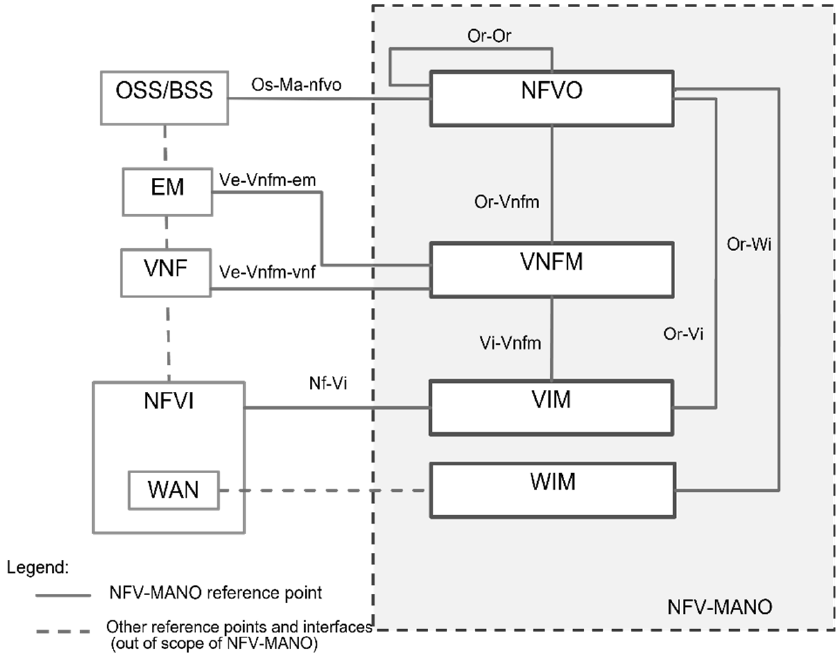
\includegraphics[width=1\linewidth]{figs/NFV-MANO-architecture.png}
    \caption{NFV-MANO architectural framework~\cite{ETSI_GS_NFV_006_V5_2_1}}
    \label{fig:nfv-mano-architecture}
\end{figure}

\clearpage

Over the years, multiple open source \acs{MANO} solutions, compliant with \acs{ETSI} \acs{NFV-MANO} have been implemented, such as the \acs{ETSI}  \acs{OSM}~\footnote{https://osm.etsi.org/}. By leveraging interfaces as the \acs{NFV}-SOL 005, it provides \acs{REST} \acsp{API} necessary for the integration with \acs{OSS}/\acs{BSS} systems, such as \acf{OSL}. This allows a more coordinated and integrated approach, yielding a series of benefits. The integration between \acs{NFV-MANO} and \acs{OSS}/\acs{BSS} systems and their benefits is further explored in Section~\ref{sec:oss:bss:nfv-mano}.





\section{5G SBA} \label{sota:sba}


The \ac{3GPP} specification for the \ac{5G} system architecture is defined to support data connectivity and services across a wide range of heterogeneous applications with diverse requirements. The 5G System adopts a \ac{SBA} with a modular and stateless \ac{NF} design, which segregates \ac{UP} and \ac{CP} functions for independent scalability and evolution. This architecture facilitates flexible deployment, where authorized \acp{NF} can access each other's services through reusable service procedures. The \ac{3GPP} TS \text{23.501} specification also identifies, among other key aspects, support for a unified authentication framework, discussed in Section \ref{sota:initiatives:CAPIF}, as well as analytics and capability exposure functionality, for third-party access, the latter of which will be analyzed in this section~\cite{ETSI_TS_123_501_V16_9_0}.

Figure \ref{fig:5g-sba} depicts the service-based representation of version \text{18.11.0} Release 18 of the Non-Roaming 5G System Architecture~\cite{ETSI_TS_123_501_V16_9_0}. It includes service-based interfaces (e.g. Nnef) for network function interaction within the \acl{CP}, as well as point-to-point reference points (e.g. N1) for interactions with \acl{UP} functions and entities (i.e \ac{UE}, (R)AN, \ac{UPF} and \ac{DN}).

\begin{figure}[htbp]
    \centering
    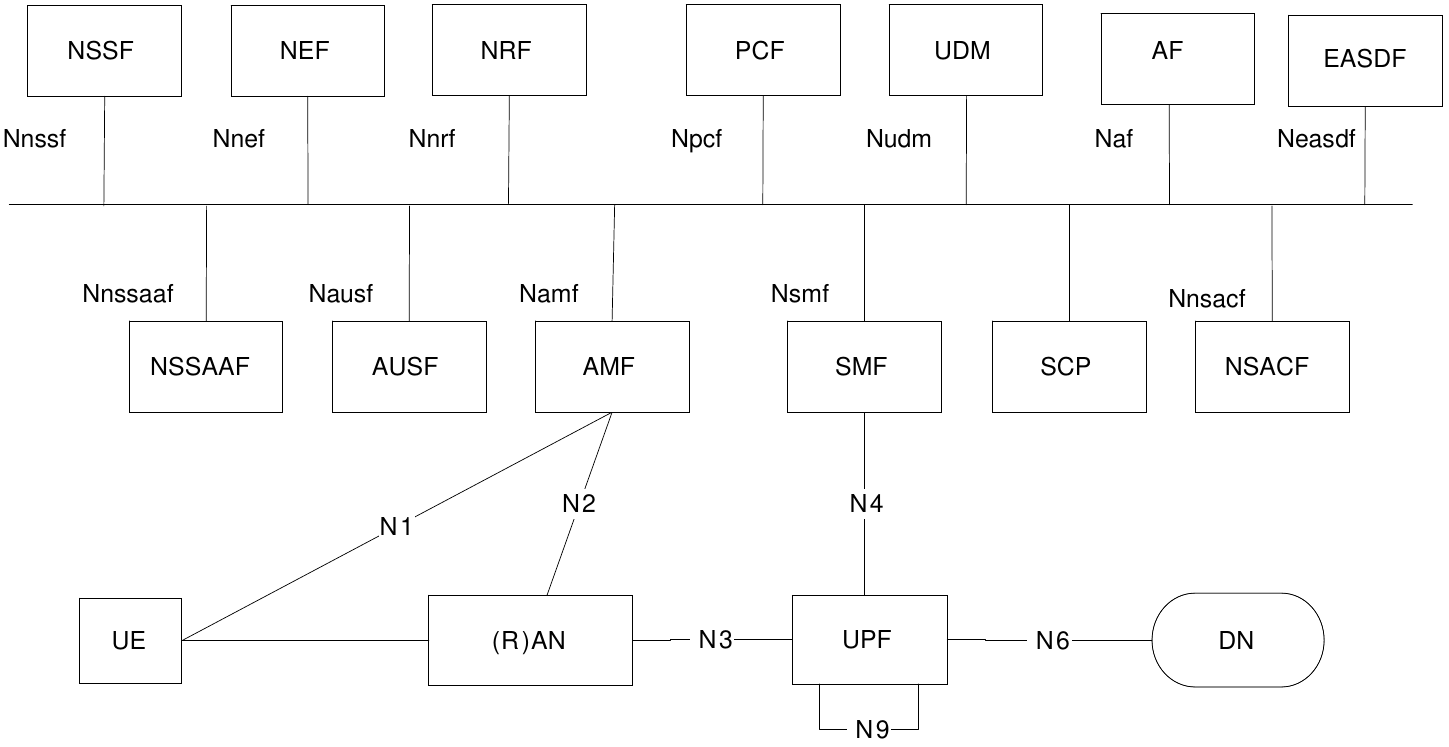
\includegraphics[width=1\linewidth]{figs/5G-SBA.png}
    \caption{Non-Roaming 5G System Architecture~\cite{ETSI_TS_123_501_V16_9_0}}
    \label{fig:5g-sba}
\end{figure}

\clearpage

The 5G System architecture consists of the following network functions:

\begin{itemize}
    \item{\textbf{(Radio) Access Network ((R)AN):}} access network that provides \ac{UE} connectivity to the \ac{5GC} Network, including NG-RAN and/or non-3GPP access technologies;

    \item{\textbf{\acf{DN}:}} external data network that provides access to operator services, third-party services or the Internet;

    \item{\textbf{\acf{AUSF}:}} supports authentication for both, 3GPP access and non-3GPP access (untrusted access via \acs{N3IWF}, trusted access via \acs{TNGF} and wireline access via \acs{W-AGF}). Its most significant functionalities include providing, to requester \acs{NF}, \acs{UE} authentication and protection mechanisms for \ac{SoR} information and \acs{UE} parameter updates;

    \item{\textbf{\acf{SMF}:}} handles \ac{PDU} session management (establishment, modification and release) and \ac{UE} \ac{IP} address allocation, including selecting and controlling the \ac{UPF} to steer traffic to the proper destination; 
    
    \item{\textbf{\acf{AMF}:}} responsible for registration, connection, reachability and mobility (e.g. handover) management between the \ac{UE} and the network. It also acts as an intermediary transport forwarding \ac{SM} messages between \acp{UE} and the \ac{SMF};

    \item{\textbf{\acf{PCF}:}} governs network behaviour based on a unified policy framework by providing policy rules to control plane functions that enforce them throughout the network. These policies cover, for example, charging, \acs{QoS} and network slicing scenarios (e.g. limits data rate per network slice). To facilitate these decisions, the \acs{PCF} accesses relevant subscription information from the \acs{UDR}, both located in the same \acs{PLMN}\hide{\later{explain this somewhere and PLMN too}};

    \item{\textbf{\acf{NSSAAF}:}} responsible for authentication and authorization mechanisms specific to a slice;

    \item{\textbf{\acf{NEF}:}} provides secure exposure of \acs{NF} capabilities and events to third parties, \acsp{AF} and edge computing environments, allowing them to interact with the network through standardized interfaces. It manages the secure provisioning of information from external applications to the internal network (e.g. authentication, authorization and assist in throttling \acsp{AF}), handling the necessary translation of data between the two domains (e.g. masking of network and user sensitive information to external \acsp{AF}'s according to the network policy). By interacting with other \acsp{NF}, namely the \acs{NWDAF}, NEF supports the exposure of \acs{NWDAF} analytics to external parties, mediating the collection of data by the \acs{NWDAF} and forwarding requests and notifications between it and the \acs{AF};

    \item{\textbf{\acf{UDM}:}} handles subscription management and access authorization based on subscription data (e.g. roaming restrictions). It is also responsible for registering and storing the \acp{NF} actively serving \acp{UE} (e.g. \ac{SMF} registration with the \ac{UDM} upon establishment of a \ac{PDU} session), which is specially relevant for service continuity (e.g. tracking \ac{SMF}-\ac{DNN} assignments of ongoing sessions);

    \item{\textbf{\acf{UPF}:}} provides an interconnection point through which external \ac{PDU} sessions connect to the \ac{DN}, handling packet routing and forwarding, such as uplink traffic between \acp{UE} and an instance of a \ac{DN}. It's also responsible for handling \ac{QoS} and policy rule enforcement within the user plane;

    \item{\textbf{\acf{AF}:}} interacts with the \ac{CN} to provide services, influencing aspects such as traffic routing, \ac{QoS} (e.g. request \acs{AF} session with required \ac{QoS}), policies and charging. Based on the deployment, \acsp{AF} considered to be trusted by the operator, as represented in Figure \ref{fig:5g-sba}, can interact directly with the rest of \acsp{NF}, whereas untrusted \acsp{AF} are required to access network function capabilities through the \acs{NEF};\hide{\later{maybe give examples}}

    \item{\textbf{\acf{SCP}:}} supports indirect communication between \acp{NF}' services, forwarding and routing messages either to the destination NF service or to a subsequent-hop \ac{SCP}. It also ensures communication security, as well as load balancing, monitoring, and overload control;

    \item{\textbf{\acf{NRF}:}} supports service decovery, allowing \acp{NF} to discover other \acp{NF} and their services, as well as SCP discovery by other SCPs. It achieves this by maintaining the current health status and profiles of available \ac{SCP} instances and \ac{NF} instances and their supported services. Additionally, it notifies subscribed consumers whenever a \ac{NF} or \ac{SCP} instance is registered, updated, or deregistered;

    \item{\textbf{\acf{NSSF}:}} responsible for selecting the Network Slice instances serving a specific \ac{UE}, tailored for specific service requirements. This includes determining the \ac{NSSAI} and, if needed, the mapping to the subscribed \acp{S-NSSAI};

    \item{\textbf{\acf{NWDAF}:}} collects and analyses data from the \ac{5G} network, leveraging information obtained from \acp{NF} (directly or via \ac{NEF}) and \ac{OAM} systems, with the goal of optimizing the 5G network's operation and service quality. \ac{NWDAF} consumers, i.e. \ac{5GC} \acp{NF} and \ac{OAM}, use the data analytics provided by the \ac{NWDAF} to assess, inter alia, slice's load level information, observed service experience, \ac{NF} load, network performance (e.g. \ac{gNB} status and resource usage) and \ac{QoS} Sustainability (e.g. \ac{QoS} change statistics). Analytics information are either statistical information on past events or predictive information (e.g. \ac{NF} load or network performance predictions, likelihood of a \ac{QoS} change) and can be obtained through the use of \ac{ML} models~\cite{ETSI_TS_123_288_V18_11_0}.

    

    % Lacks EASDF, NSACCF

\end{itemize}

\hide{

mention virtualization and softwarization

NFV and SDN

transition to a software-driven architec-
ture, emphasizing virtualization and cloud technologies, and
adopted a Service-Based Architecture (SBA) for scalable and
modular Network Functions (NFs)

scalable evolve indepedntly
}

\subsection{Network Analytics Capabilities}

The introduction of \ac{NWDAF} and its data collection, analytics and predictive capabilities, unlocks the possibility for data-driven network solutions that automate network management and optimize resource allocation~\cite{AdvancingPredictiveSecurity}. Capitalizing on this potential, several studies in the literature have explored various use cases for the \ac{NWDAF}, including solutions in network security and threat mitigation, as well as resource and operational efficiency. In the context of network security and threat mitigation, \ac{NWDAF} can, from collected data from functions such as the \ac{SMF}, \ac{AMF}, \ac{AF} and \ac{UPF}, identify abnormal user behavior and specific types of \ac{DDoS} attacks detecting UDP fragmentation, SYN, ICMP, DNS, and GTP flood attacks~\citep{AdvancingPredictiveSecurity,UserTerminalsAsAttackers}. This \ac{NWDAF} functionality can be extended to any anomaly detection scenarios in sectors such as logistics, maritime, and smart cities, where it can monitor communication patterns from vehicles, vessels or \ac{IoT} sensors to identify irregularities indicative of hijacking, system malfunctions or cyber-attacks~\cite{UserTerminalsAsAttackers}. Regarding resource and operational efficiency, the \ac{NWDAF} is capable of analysing \ac{RAN} data, \ac{UPF} traffic and CPU usage to predict network load and resource utilization, and proactively allocate additional resources when necessary, preventing performance degradation with faster response times than a simple threshold-based strategy~\cite{ExplorationNWDAFDevelopmentArchitecture6G}.


Additionally, the operation of the \ac{NWDAF} in conjunction with other \aclp{NF}, namely the \acs{NSSF}, supports automatic slice selection mechanisms with data collected and analysed by the \ac{NWDAF}. By evaluating \acs{QoS} and \acs{QoE} metrics and leveraging machine learning models, the network can dynamically select the most suitable vertical slices, acommodating a variety of \ac{IoT} use cases such as vehicular or real-time health systems~\cite{NetworkSliceSelectorIoT}.

\subsection{Network Exposure Capabilities} \label{sec:network:exposure:mechanisms}

The exposure of network capabilities has introduced a new level of flexibility for users and applications, allowing them to leverage and influence the capabilities of the network rather than being constrained by the functionalities explicitly offered by the mobile network. By granting access to third party external applications, this also opens the possiblility for telecom \acsp{SP} to monetize their network capabilities. With this objective, 3GPP has specified a series of Capability Exposure frameworks through the use of Northbound \acsp{API} and Application Enabler Layer \acsp{API}~\cite{CapabilityExposure3GPP}.

\subsubsection{\acl{NEF}} \label{sec:sba:nef}

The core network function responsible for \acs{5G}'s network capability exposure is the \acs{NEF}. The \acs{NEF} securely exposes \acsp{NF}' capabilities to external third parties, providing a set of northbound \acsp{API} through which they can interact with the \ac{5GC} to build network-aware applications. Thus, the \acs{NEF} allows service providers to access network capabilities contributing to the concept of an open and programmable network, while abstracting them from the underlying network~\cite{NEFsim}. More specifically, \acs{NEF} offers an exposure layer composed of northbound \acsp{API}, which are then internally connected to the \acs{SBA} southbound \acsp{API} to provide the intended functionalities, such as exposing network data and receiving management commands~\cite{CAPIFmicroserviceVerticals}. This and all other exposure capabilities supported by the \acs{NEF} can be classified into the following categories~\cite{ETSI_TS_123_501_V16_9_0}:
\begin{itemize}
    \item \textbf{Monitoring capability:}  monitoring of specific \acs{UE} events in the \acs{5G} System and making the correponding event information available for external exposure via the \acs{NEF}. Monitoring capability supports exposing \acs{UE}'s mobility management context such as \acs{UE} location, reachability, roaming status and loss of connectivity, as well as \acs{QoS} monitoring results. It includes functionality for identifying the \acs{5G} network function most suitable for configuring the specific monitoring events, detecting the monitoring event and reporting it to the authorised external party;
    
    \item \textbf{Provisioning capability:} allows an external party to provision information that can be used for the \acs{UE} in the \acs{5G} System. Provisioning Capability permits the external party to provision Expected \acs{UE} Behaviour, \acs{5G-VN} group information or service specific information to a \acs{5G} \acs{NF}. It comprises of the authorisation of the provisioning external third party, receiving the provisioned external information via the \acs{NEF} and storing and distributing it to the requiring \acsp{NF};
    
    \item \textbf{Policy/Charging capability:}  handling access and mobility management, \acs{QoS} and charging policies for the \acs{UE} based on a request from an external party. More specifically, it has mechanisms for handling a specific \acs{QoS}/priority setting for an \acs{UE} session and configuring the applicable charging party or charging rate;
    
    \item \textbf{Analytics reporting capability:} enables an external party to fetch, subscribe or unsubscribe to analytics information generated by the \acs{5G} System. Analytics reporting capability incorporates functionality for discovering the type of analytics available to an external party and requesting analytics information generated by the \acs{NWDAF} for consumption;

    \item \textbf{Member \acs{UE} selection capability:} allows an external party to acquire one or more list(s) of candidate \acs{UE}(s), selected from the list of target member \acs{UE}(s) provided by the \acs{AF}, along with additional information derived from assistance information generated by the \acs{5G} System based on predefined filtering criteria.

\end{itemize}


\subsubsection{Application Enabler Layer}

Unlike the previous generations, \acs{5G} focuses on enabling vertical applications integrated with the underlying \acs{5G} network, potentially providing \acsp{MNO} with new revenue streams and shifting away from traditional \acf{B2C} models, with an end-user, toward \acf{B2B} opportunities, with industry verticals~\cite{SEAL5GVerticals}. To capitalize on the monetization of their network capabilities while tailoring to the needs of the various vertical sectors, 3GPP has defined capability exposure frameworks based on Application Enabler Layer \acsp{API}. 

Application Enabler Layer \acsp{API} are abstraction layers for specific vertical applications (e.g. Edge, \acs{UAS}, {V2X}) or common to multiple vertical applications, which allow the exposure of common core and application enabler services to external applications. This abstraction is provided in paralell or on top of abstraction functionalities already provided by Network Northbound \acsp{API} via the \acs{NEF} or any other network \acsp{API} (e.g. network management \acsp{API}) to fullfill requests from vertical applications~\cite{CapabilityExposure3GPP}.

The Application Enabler Layer \acsp{API} designed to be common for multiple vertical applications are securely provided to verticals through the \acf{SEAL}~\cite{ETSI_TS_123_434_V18_12_0_SEAL}. The \acs{SEAL} defines a standardized functional architecture considering the common capabilities required to support multiple vertical applications over 3GPP networks. These capabilities are accessible for use through the following \acs{SEAL} services: Location management, Group management, Configuration management, Identity managemen, Key management, Network resource management, Data delivery, Notification management, Network slice capability enablement and Application data analytics enablement~\cite{ETSI_TS_123_434_V18_12_0_SEAL}. Many of these capabilities correspond to auxiliary services that address cross-cutting concerns, common across verticals. Developing them independently for each vertical would be redundant and require substantial time and effort. Instead, vertical application developers can focus exclusively on the core features and functionalities of the vertical application, while utilizing \acs{SEAL} for the auxiliary services, thus saving significant time and cost to market~\cite{SEAL5GVerticals}.

In addition to \acs{SEAL}'s common reusable services across multiple vertical sectors, a dedicated service framework is required to address the specific requirements of edge-based services and edge computing. Edge Computing is a network architecture concept that deploys cloud computing capabilities and service environments close to the \acsp{UE}, with the goal of achieving several benefits, such as lower latency, higher bandwidth, reduced backhaul traffic and possibly new innovative services not feasible or supported in regular cloud environments. With this goal, 3GPP specifies an application architecture for enabling Edge Applications on the \acf{EDN}. More specifically, it introduces the \acf{EEL} to facilitate communication between the \acfp{AC} running on an \acs{UE} and the \acf{EAS} deployed on the \acs{EDN}. Regarding network exposure capabilities, the \acs{EEL} exposes northbound \acsp{API} towards the \acsp{EEC} (running on an \acs{UE}), \acsp{EAS} (possibly third-party \acsp{EAS} outside the \acsp{ECSP} trust domain) and other internal functional entities. These services encompass native \acs{EEL} services, such as service provisioning, \acs{EAS} discovery and support for service continuity, as well as enhanced re-exposed services of the 3GPP \acs{CN}, such as \acs{UE} Location and \acs{QoS} sessions. While distinct in their application, both categories utilize the exposed network capabilities via \acs{NEF} northbound \acsp{API}, optionally via \acs{CAPIF}. Native services consume these network capabilities to support internal logic, such as retrieving a \acs{UE}'s location to filter discovery results, whereas re-exposed services are built directly on the \acs{NEF} capabilities to provide enhanced access to network functions~\cite{ETSI_TS_123_558_V18_11_0_EDGE}.

The previously mentioned enabler layers focus on generic application support for multiple vertical applications and edge applications, respectively. To address the diverse requirements of heterogeneous vertical use cases, additional vertical-specific enabler layers were defined. The \acf{VAE} layer ensures efficient use and deployment of \acs{V2X} applications on 3GPP networks, supporting use cases such as platooning, remote and tele-operated driving, \acs{HD} maps and Vehicle-to-Pedestrian communication with \acf{VRUP}. It serves as an abstraction layer that encapsulates the underlying mechanisms from the \acs{V2X} application specific layer and exposes them via northbound \acsp{API}, providing interfaces for operations such as group management and message distribution. To support these functionalities, the \acs{VAE} utilizes the \acs{NEF} for interacting with the \acs{5G} System, allowing it to receive \acs{QoS} monitoring information and network data analytics (e.g. congestion status reported by the \acs{NWDAF} to \acs{NEF}). It also relies on \acs{SEAL} for support services in location management, group management, configuration management, identity management, key management and network resource management, thus emphasizing the importance of these components in the \acs{V2X} vertical-specific scenario~\cite{ETSI_TS_123_286_V19_0_0_V2X}.

Similar enabler layers exist for other vertical sectors in \acf{UAS}~\cite{ETSI_TS_123_255_V18_2_0_UAS}, \acs{5G} messaging for \acf{MIoT} communication~\cite{ETSI_TS_123_554_V18_10_0_Messaging} and \acf{FF}~\cite{3GPP_23_745_V17_0_0_FF}. All provide abstraction layers for vertical specific capabilities, exposing northbound \acsp{API} that may require interactions with the \acs{NEF} and \acs{SEAL} components to fulfill these capabilities, optionally via \acs{CAPIF}.



\subsubsection{NEF Implementations} \label{exposure:NEFimplementations}

In regards to \ac{NEF} implementations, there are a variety of implementations across both open source 5G core solutions and in commercial deployments. This section provides an overview of the current \ac{5G} \ac{NEF} solutions and their supported northbound \acsp{API} and services, followed by a discussion of their level of adoption in the literature. 

Concerning commercial solutions, Nokia's \ac{NEF}~\cite{NokiaNEF2022} is described as a cloud native \ac{PaaS} following a microservices architecture with a \ac{REST} aproach. However, proprietary commercial solutions are constrained by licensing restrictions, making free and open-source alternatives more viable.

As for open source projects, the presence of the \ac{NEF} component varies across different \ac{5G} core implementations. For instance, Open5GS, despite providing a C-based implementation of a \ac{5G SA} Core with a \ac{SBA} architecture supporting a wide variety of network functions, it still lacks a \ac{NEF} implementation~\cite{Open5GSDocs}. Consequently, authors have resorted to extending the Open5GS \acs{CN} by developing and integrating their own \ac{NEF} solutions~\citep{CloudEnabledDeployment5GN, DynamicQoSAdaptationviaExposedServiceAPIs}. The \ac{5G} \ac{CN} provided by the \ac{OAI} software alliance does not provide \ac{NEF} functionality either, with support expected in a future release scheduled for the first semester of 2026~\cite{OpenAirInterface5GCN}. In constrast, Free5GC, by the Linux Foundation, includes a partial \ac{NEF} implementation~\cite{Free5GC-NEF}, enabling exposure of network capabilities through services such as \texttt{Nnef\_PFDManagement} and \texttt{Nnef\_TrafficInfluence}, as defined in 3GPP TS 23.502~\cite{3GPP-23.502}. However, certain inconsistencies exist, notably regarding traffic steering capabilities via the \ac{NEF}, which are available in version 3.4.5 but absent in version 4.0.0~\cite{Free5GCv4.0.0NotSupportTrafficSteering}.

% Nnef\_PFDManagement       -> PfdManagementAPI     (TS 29.122)
% NNef\_TrafficInfluence    -> TrafficInfluenceAPI  (TS 29.522)

However, to the author's best knowledge, the level of adoption to actual \ac{NEF} implementations remains relatively low in the research community, at least in the researched body of literature considered in this dissertation. Despite the first release of Free5GC's \ac{NEF} being introduced on 12 November 2024, subsequent research papers in 2025 still do not utilize this implementation~\cite{LoadBalancingConnectedVehicleServices}\hide{\later{only one paper for this, should be at least 2}}, instead extending the \acs{CN} with custom \ac{NEF} solutions.

An alternative approach to these implementations is the open-source \ac{NEF} simulator NEFSim~\cite{NEFsim}, developed under the European project EVOLVED-5G. The component offers the standardized set of NEF northbound \acsp{API}, allowing their validation in a configurable and simulated environment. This proves especially valuable for testing and validation purposes aiding Network App developers to integrate \ac{NEF} clients into their applications, without requiring access to a full-blown \ac{NEF} instance. Thus, as the \ac{NEF} constitutes the main gateway to the \ac{5G} System, proper interaction with the \ac{NEF} ensures that Network Applications can also correctly interact with the \acs{5G} System~\cite{AutomatedTestingOrchestrationFramework}. The current implementation, extended at \acs{ITAv}, supports the PfdManagement, MonitoringEvent, AsSessionWithQoS and TrafficInfluence \acsp{API}, as per the \acs{3GPP} TS 29.522 northbound \acs{API} specification~\cite{ETSI_TS_129_522_V18_11_0}. Therefore, the NefSim supports a broader set of \acs{NEF} northbound \acsp{API}, as summarized in Table \ref{tab:nef:comparision:short}. This corresponds to a condensed version, with the full comparison encompassing all \acs{NEF} northbound \acsp{API} being presented in Table \ref{tab:nef:comparision:long} of the Appendix \ref{chap:appendix-more}. Additionally, among the analysed open-source implementations it is the only one that features \acs{CAPIF} integration, significantly reducing integration effort on adoption. 

\begin{table}[ht]
\centering
\renewcommand{\arraystretch}{1.3} % Increase row height
\rowcolors{2}{gray!15}{white}     % Alternating row colors
% Implemented ?
% $\checkmark$      -> yes
% $\times$          -> no
% $\LEFTcircle$     -> partially
\begin{tabular}{p{6cm} c c c}
\toprule
\textbf{Northbound \acs{API}} & \textbf{Free5GC} & \textbf{NEFSim} \\
\midrule
% Implemented ?
% $\checkmark$      -> yes
% $\times$          -> no
% $\LEFTcircle$     -> partially
PfdManagement                & $\checkmark$         & $\checkmark$ \\
MonitoringEvent              & $\times$             & $\checkmark$ \\
AsSessionWithQoS             & $\times$             & $\checkmark$ \\
TrafficInfluence             & $\checkmark$         & $\checkmark$ \\
\bottomrule
\end{tabular}

\caption{Northbound API Coverage across open source NEF Implementations}
\label{tab:nef:comparision:short}
\end{table}




\hide {

\later{Observation in other paper (cloud-native NEF and CAPIF interplay) regarding NEFSim: Still, NEFSim does not allow interacting with a CN or southbound, or refer to CAPIF. -> I also don't understand which NEF they actually use}

GIRL
- openness by enabling new levels of programmability in the core and edge
domains, which allows third-party innovators, also known as vertical industries, to control and monitor the deployment process and performance of their services
- securely made through the NEF's APIs, hiding all the underlying network topology, to external third parties that may use them to build network aware applications
- northbound APIs

OTHERS
cloud-enabled deployment of 5G Core network with analytics features -> However, NEF is not included in the most popular open source implementations of the 5GCN (OPEN5GS doesn't have NEF implemented)

(load-balancing-in-connected-vehicle) UERANSIM [18] for simulating UE and gNB.

}

\section{Network Applications} \label{sota:networkapplications}

Network Applications, were first described in 2019 at the 5GPPP Horizon ICT-41-2020 calls, as a concept to chain \acp{VNF} across several domains to create applications tailored to the requirements of specific tenants or verticals. Under this initial proposal request, particular emphasis is placed on the creation of open platforms for development, testing and validation of network applications according to each specific vertical use case. By utilizing these experimental facilities, third parties such as \acsp{SME}, service providers or target vertical users would be able to experiment and test their applications in fully featured virtualised 5G infrastructure, in the context of specific vertical sectors including connected and automated mobility, smart factories and industry 4.0~\cite{ICT-41-2020}.

The concept of network applications lacks a common standard definition, with various organizations and standardization bodies offering slightly different interpretations depending on their specific context.

From a technical testing and validation perspective, \acs{ETSI} simply defines it as "a virtual application that can be deployed in a 5G infrastructure and can use 5G services" (e.g., connectivity or localization). In this interpretation, a network application is composed by one or more \acp{AF} or \acp{NF} (not to be confused with components from \ac{5G} \ac{SBA}), responsible for implementing the application logic and the underlying network/communication functionalities, respectively. Each of these individual components can either be statically deployed on top of physical hardware or through virtualization techniques, i.e. virtual machines or cloud-native containers~\cite{ETSI_TS_104_074_V1_1_1}.

The 5G-PPP Software Network Working Group further refines this definition as a collection of services that provide certain functionalities to verticals and their associated use cases by interacting with the mobile network's control plane through exposed Open \acsp{API}, such as \acs{5GC} northbound \acsp{API} (e.g. via \acs{NEF}), the \acs{RIC}, and edge computing \acsp{API}. In their view, Network Applications provide a middleware layer between verticals and \acsp{CSP} that simplifies the implementation and deployment of vertical systems at large scale, allowing contribution from third parties or network operators based on the established level of interaction and trust. The document also specifies a set of optional requirements that characterize a network application, including its ability to span one or more \acs{5G} network slices and to consume monitoring and telemetry data from the \acs{5G}/\acs{B5G} system to support analytics and operational functions~\cite{NetworkApps5GPPP}.

An even more granular and nuanced definition is provided by \citet{CAPIFmicroserviceVerticals}, with emphasis on guaranteeing a secure, standardized and trusted access to the aforementioned \acsp{API}, through required standardized \acs{CAPIF} compliance.

For the purposes of this dissertation, the definition of Network Applications proposed by the 5G-PPP is adopted due to being the most complete. However, this definition could be completed further, emphasizing alignment with telecom standardization initiatives, such as \acs{CAPIF} for secure capability exposure, and the CAMARA project for establishing standardized user-friendly network \acsp{API}. Combined, these initiatives enable new interaction models with the control plane of the \acs{5G} core, supporting the fulfillment of network application use cases.


\hide{
(WHY IS TESTING / VALIDATING NETWORK APPLICATIONS IMPORTANT)


não é só network applications mas sim interfaces e todo o tipo de cenas relacionadas a 5G

not only from the vertical perspective but also from the 

CAPIF paper -> Using CAPIF terminology, NetApps are, by nature, API
Invokers that consume APIs exposed by AEFs. 

}

\subsection{Use Cases} \label{sota:networkapplications:usecases}

Following the conceptual definition of network applications, this section outlines their diverse array of use cases implemented throughout the literature. A frequently addressed use case corresponds to \ac{CAM} scenarios, with a particular emphasis on digital twin implementations. \citet{VirtualOnBoardUnitMigration} focus on a network application that supports the creation of digital twins for physical \acsp{OBU} placed in modern vehicles. These v\acsp{OBU} follow the vehicle by automatically migrating between different \ac{MEC} domains to maintain low-latency access, while facilitating collection and offloading of the vehicular sensor data to the edge. In the context of \acs{CAM} vertical use cases, subsequent research further explores the digital twin concept, emphasizing the use of \ac{QoS} profiles to guarantee sufficient data throughput for vehicular data collection on congestioned areas based on vehicle location~\cite{DynamicQoSAdaptationviaExposedServiceAPIs}.

A similar concept can also be applied to the \ac{T&L} sector, particularly to enhance safety and efficiency of remote vessel operation in busy port environments. \citet{NextGenConnectivityDynamicQoS} introduce the concept of Edge Network Applications (EdgeApps), which interact with the \acs{5G SA} network to dynamically modify \acf{QoS} based on vertical needs. More specifically, it proposes two EdgeApps: the Situational Awareness EdgeApp and the Quality Awareness EdgeApp. The Situational Awareness EdgeApp dynamically adjusts network \acs{QoS} based on the vessel's context and location, such as entering busy port areas or bridges, guaranteeing an higher bandwitdh or uplink capacity to ensure safe and efficient remote operation. It is also responsible for reducing the load on the network in scenarios where high-quality video streams are not needed: vessels operating in fully autonomous mode or manually controlled onboard. The Quality Awareness EdgeApp actively monitors the link network quality (performance), detecting when the network is under-performing, triggering \acs{QoS} adjustments or notifying the remote captain if necessary.

Beyond vehicular scenarios, network applications have also been explored in the context of media and streaming, where maintaining a high level of \ac{QoE} across high traffic and variable network quality is critical. The work by \citet{BenefitsCaveatsQoDNetworkAPIsVideoStreaming} investigates the use of a \ac{CDN}  to improve the \ac{QoE} amidst difficult network conditions by providing additional network bandwidth to a given video streaming session, according to a predefined strategy (e.g. based on the buffer length).

Finally, a comprehensive list of 11 network applications that were tested and certified under the 5GASP project in 2024 is also available~\cite{NetApps5GASP}, among which particular attention is given to those targeting public safety and \ac{PPDR} scenarios: \ac{5G} \ac{IOPS}; \ac{FIDEGAD}. The \ac{IOPS} network application aims to maintain a level of communication between public safety users (e.g. emergency responders), ensuring continuity of mission-critical services in situations where the backhaul connectivity ot the core network is not fully functional or disrupted, such as in \ac{PPDR} disaster situations and in out-of-coverage areas~\cite{IOPS5G}. The \ac{FIDEGAD} network application is deployed on an air drone to provide the first assessment of buildings and forests affected by fire. The network application handles the drone's live image streaming, transmitting telemetry and sensor data through the \ac{5G} system to ground teams, while performing the necessary handovers between \ac{5G} stations~\cite{FIDEGAD5G}.

\hide{

-> coupled with IoT 

-> capability exposure

-> tomam partido da NSSF function (machine learning blah blah). Support wide variety of IoT use cases, such as blah blah

-> tomam partido da NWDAF function 


\later{5G-Advanced}


Edge Network Applications -> DynamicQoS Optmization for 5G Stan

 V IRTUAL O N -BOARD U NIT MIGRATION IN A
M ULTI - ACCESS S MART-C AMPUS 5G A RCHITECTURE -> NEF (Virtual On-board Unit Migration)

PPDR

\later{CHECK PAPER Service Requirements of 5G System by 3GPP}

}




\section{Key Telecom Standardization Initiatives} \label{sota:telcoinitiatives}

Section \ref{sota:networkapplications} highlights the importance of telecom standardization initiatives for the definition of network applications and the fulfillment of their use cases. This section provides an overview of the most relevant standards across the industry and academia, outlining the benefits they provide to both developers and operators. In the case of \acs{CAPIF}, this also includes a detailed description of its functional architecture and main entities involved in secure \acs{API} exposure.

\subsection{CAMARA Project} \label{sec:iniatives:CAMARA}

% connection with GSMA not present (should I mention it??)
% INTEROPERABILITY developers, operators, and enterprises

The CAMARA Project, an open-source initiative under the Linux Foundation, focuses on defining, developing and testing simplified telco \acsp{API} to access complex network functions and services. Its primary goals are: (i) simplifying telco complexity through user-friendly \acsp{API} easy to consume for customers with no telco expertise; (ii) facilitating application to network integration; (iii) supporting application portability~\cite{CAMARAProject}.

More specifically, CAMARA abstracts network complexities by presenting a cohesive taxonomy of user-friendly service \acsp{API} throughout a variety of domains, such as network slicing, \ac{QoS} and Location. CAMARA \acsp{API}, being widely adopted by major telecommunication operators and cloud providers (in conjunction with \acs{GSMA}~\cite{CAMARAGSMAindustry}), abstract developers from complex interactions with \ac{5G} Core components, such as the \ac{AMF} and \ac{LMF}, allowing them to integrate advanced network capabilities in a unified ecosystem, while solely focusing on the innovation and design of their own applications.

\hide{\later{Network as a Service -> open and programmable network}}

\subsection{GSMA Open Gateway}

%agilizar - acelerate

The \acs{GSMA} Open Gateway is an initiative lauched by \ac{GSMA} with the goal of establishing a global standardized framework of common network \acsp{API} that simplifies access to mobile operator networks. By giving developers and cloud providers a single point of access to network capabilities provided by multiple operators, \acs{GSMA} Open Gateway promotes simplified integration and service delivery, eliminating the need to individually deal with multiple different operator specific \acsp{API} and accelerating time to market. This is achieved through northbound service \acsp{API}, supported by the CAMARA Project, exposing the mobile operators' network capabilities within a consistent, interoperable and federated framework~\citep{gsmaGSMA,telefonicaGSMA}.

\hide{
6\_Optimizing\_3GPP\_5G\_NEF\_Integration\_Enhancing\_Programmable\_Networks\_Through\_NEF\_and\_UPF\_Interoperability -> abstraction of complexity, introducin CAMARA, CAPIF, reduce time to market 
}

\subsection{CAPIF} \label{sota:initiatives:CAPIF}

% https://www.3gpp.org/technologies/ct3-exp-fr-apis
% https://www.3gpp.org/technologies/rnaa
% https://www.3gpp.org/news-events/3gpp-news/sa6-verticals2

\hide{\later{mention SEAL and NEF support for CAPIF in 5g sba spec (ETSI SPEC)}}


The \acf{CAPIF}, specified by \ac{3GPP}, establishes a single exposure platform for all \ac{3GPP} capability exposure \acsp{API} and non-\ac{3GPP} defined \acsp{API}. The first category includes: (i) Network Northbound \acsp{API} for secure exposure of the \ac{3GPP} core network to external applications via the \ac{SCEF} or \ac{NEF} functions, for \ac{4G} and \ac{5G}, respectively; (ii) Application Enabler Layer \acsp{API} which provide enabler abstraction layers for exposure of common core and application enabler services to external applications. The latter comprises of \acsp{API} defined by other \acs{SDO} or consortiums such as \acs{TMF} or CAMARA~\cite{CapabilityExposure3GPP}. % websites

% Paper CAPIF Microservice & Website
\acs{CAPIF} offers common supporting functionalities applicable to any service \acsp{API} at the northbound of a mobile network. These include on-boarding and off-boarding of \acs{API} invokers, registering and releasing \acsp{API} for exposure and \acs{API} authentication, authorization and discovery by third-parties. This unified framework simplifies and accelerates the delivery of applications (\ac{AF}s) invoking \acsp{API}, while preventing duplication and inconsistences across existing \acs{API} specifications. Furthermore, by allowing third parties to define and publish their own \acsp{API} and securely access 5G core \acsp{API}, CAPIF promotes Network Openness towards Verticals~\cite{CAPIFmicroserviceVerticals}. These capabilites have been fundamental in 3GPP SA6 for facilitating Vertical interaction with the 5G System~\cite{CAPIFSA6}.

% CAPIF ETSI White Paper CAPIF Microservice
% falar dos vários componentes e da arquitetura!!

The \ac{CAPIF} architecture is illustrated in Figure ~\ref{fig:capif-architecture}. It is constituted by three main entities: the \ac{CCF}, the \acs{API} Invoker and the \acs{API} Provider. A brief description of each of the entities and its responsabilities is provided bellow~\citep{CAPIFmicroserviceVerticals,ETSI_CAPIF_TS_123_222_V18_4_0}.

\clearpage


\begin{figure}[htpb]
    \centering
    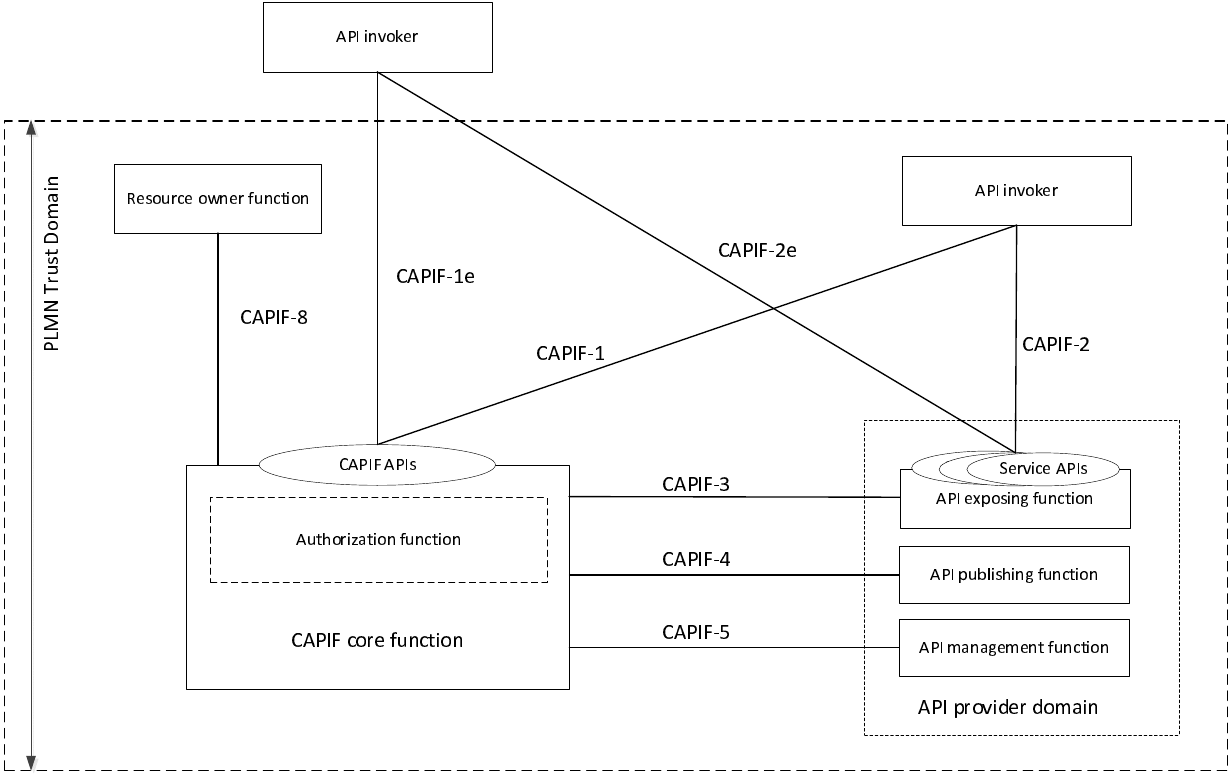
\includegraphics[width=1\linewidth]{figs/capif-architecture.png}
    \caption{High level functional architecture for CAPIF supporting \acs{RNAA}~\cite{ETSI_CAPIF_TS_123_222_V18_4_0}}
    \label{fig:capif-architecture}
\end{figure}


\customparagraph{API Invoker}

The \acs{API} Invoker is typically provided by a third-party application, on a server or \acs{UE}, who has a service agreement with the \acs{PLMN} operator. The \acs{API} Invoker may reside within or outside the \acs{PLMN} operator trust domain and has the following main goal: triggering its onboarding/offboarding and authentication with \acs{CAPIF}, discovering available service \acsp{API} and invoking those \acsp{API} to access network or service capabilities. 

\customparagraph{API Provider}

The \acs{API} Provider represents an entity that owns and exposes \acsp{API} to the \acs{API} Invokers through the CAPIF framework. It provides three different functions: \ac{CAPIFAEF}, \ac{CAPIFAPF} and \ac{CAPIFAMF}.

The \ac{CAPIFAEF} is the service \acs{API} provider and communication entrypoint to the \acs{API} Invokers, handling its authentication and validating the authorization provided by the \ac{CCF} via \acs{JWT}. It is also responsible for logging the service \acs{API} invocations at the \ac{CCF}. The \ac{CAPIFAPF} allows \acs{API} providers to publish their service \acs{API} information to the \ac{CCF} in order to support \acs{API} discovery by \acs{API} invokers. The \ac{CAPIFAMF} lets the \acs{API} provider perform administration of the service \acs{API} including auditing service \acs{API} invocation logs and  monitoring events from \ac{CCF}. It also allows the \acs{API} provider to configure policies to the \ac{CCF}, between other capabilities.

\customparagraph{CAPIF Core Function}

The \ac{CCF} is the core component and acts as the central repository for all published \acsp{API}, controlling service \acs{API} access based on \acs{PLMN} operator configuration policies and handling aspects related to storing (logs provided by the \ac{CAPIFAEF}), auditing, charging and monitoring service \acs{API} invocations. Related to the \acs{API} invoker it is responsible for its onboarding/offboarding, authentication and authorization prior to it accessing the service, as well as publishing, storing and supporting the discovery of service \acs{API} information. In the context of a 4G or 5G system, the \ac{CAPIFAEF} corresponds to the \ac{SCEF} or \ac{NEF} functions.

Lastly, with the goal of \acs{CAPIF} supporting \ac{RNAA} two additional functions are defined: the authorization function and a resource owner function. The former is an internal entity of the \ac{CCF} and interacts with the \ac{CAPIFAEF}, which acts as a resource owner consent enforcement point. The latter interacts with the authorization function via CAPIF-8, which is not specified in the current release of the specification.

\hide{

\later{
\later{TS 33.501}
The security aspects of \acs{CAPIF} supporting RNAA are specified in 3GPP TS 33.122 [12].} \later{The API invoker interacts with authorization function in the CAPIF core function via CAPIF-1/CAPIF-1e.} \later{add diagram and all connections} \later{sequence diagram flow} \later{different authentication mechanisms} \later{add reference to pathway\_towards\_NaaS\_CAMARA.pdf which includes CAPIF}

}


\subsection{TM Forum}
\label{sota:telcoinitiatives:tmf}


\ac{TMF}~\footnote{https://www.tmforum.org/} is a global aliance composed of telco and tech companies from the connectivity ecosystem with the goal of providing a cooperative framework to collaborate and establish industry-wide standards, best practices and toolkits. These include over 800 organizations, encompassing the top 10 \ac{CSP}s, the three leading hyperscalers, major Network Equipment Providers, as well as a diverse array of vendors, consultancies, and system integrators~\cite{aboutTMF}.

The core element of \ac{TMF}'s approach in achieving its missions is the \ac{ODA}. \ac{TMF} \ac{ODA} advocates for the existence of technology agnostic Open \ac{API}s, collaboratively developed by its members to provide standardized interfaces that streamline digital services across a wide range of domains, such as \ac{IoT} or healthcare. In the telecoms industry, the Open \ac{API} Project plays a crucial role in gathering \ac{CSP}s and solution and technology providers to accelerate the deployment of interoperable telecom solutions, tackling integration and delivery complexity while reducing time-to-market~\cite{openAPIsTMF}.

\ac{TMF} Open \ac{API}s rely on a common API data model that is maintained separately from the API specifications: the \ac{TMF} \ac{SID}. This model, used across the Open Digital Architecture and Open APIs, adresses the \ac{CSP}'s need for shared information definitions and models, establishing a standardized way to represent and organize data for implementing business processes. This business model is independent of platform, language or protocol and helps to identify and categorize business entities important to \ac{CSP}s, reducing duplication and promoting consistency and interoperability. More specifically, business entities can be categorized into the following domains: Market \& Sales, Customer, Product, Service, Resource, Business Partner, Enterprise and Common~\cite{SIDTMF}. Three of these domains are essential and widely used across \acfp{OSS}, such as openslice, and are explored further: the Product, Service and Resource domains.

\hide{
\later{mention relation with BSS and OSS} \later{connect with GSMA and CAMARA (i record some of page of their website mentioning it)}
}

\clearpage
\customparagraph{Product}

A Product represents a tangible or intangible item that enterprises such as \ac{SP}s expose and sell to customers for a profit. It is defined in \ac{SID} through a Product Specification detailing its attributes, methods, relationships and constraints, as perceived by the business user and aligned with what the operator intends to sell at a functional level~\cite{SID-MODELS-v250-TMF}.
% maybe other cites

\customparagraph{Service}

A Service represents internally the underlying technical implementation of a Product, which is offered to customers in a commerce perspective. Services can be categorized into \acfp{CFS}, representing, within an organization's infrastructure, the Product the end-customer acquires (e.g. a music streaming service), and \ac{RFS}, which provide the internal implementations required to support a \ac{CFS} in order to deliver its intended functionalities (e.g. recommendation engine supporting music streaming service). Each Service is defined by a corresponding Service Specification~\cite{SID-MODELS-v250-TMF}.

\hide {

\later{mention Service bundles somewhere}
\later{However, the characteristics' values of the instantiated Service will be specific to each instance.}
\later{Service specification can have multiple other service specifications}

}


\customparagraph{Resource}

Resources are the components that support the provision of Services and therefore the delivery of Products to Customers. These include Physical Resources, such as a router or server, and Logical Resources, such as Virtual Machines, \acp{VNF} or software applications, as well as Compound Resources that aggregate them into a single entity. All three Resource types are instantiated from their respective Resource Specifications, as per the specification~\cite{SID-MODELS-v250-TMF}.


\section{Management and Support Systems} \label{sota:bss-oss-mano}

The telecommunications industry is undergoing a fundamental transformation, with telecom service providers facing significant challenges as traditional networks and services become increasingly converged. Since legacy \acs{IT} systems are unable to meet the requirements of new services and customer demands, \acs{OSS}/\acs{BSS} systems, based on the eTOM framework by \acs{TMF}~\cite{eTOM-TMF}, are adopted to enable service focused operations and improve customer satisfaction. These systems serve as management platforms for telecom operators and their networks, allowing them to capitalize on new revenue streams by delivering new services to customers~\cite{NGOSSEvolutionTelecomSP}.

Their implementation is central to reducing costs and improving operational and organizational efficiency~\cite{NGOSSEvolutionTelecomSP}. By automating operational tasks, \acs{OSS}/\acs{BSS} solutions allow operators to reduce \acs{OPEX} associated with customer and system management~\cite{OSSMobileNetworks}. This is especially relevant as the number of devices connected to the network grows, with scalability heavily relying on its ability to autonomously configure, provision and update devices without impacting the network~\cite{EricsonOSS}. More importantly, the next generation of \acs{OSS}/\acs{BSS} must advance beyond traditional automation to support orchestration and dynamic allocation of network resources, setting as the ultimate goal a zero-touch network completely integrated with an orchestrator~\cite{SurveyOrchestrationOSSNextGenerationNetworks}.

\subsection{Business Support System}

The \acf{BSS} is responsible for the support of business operations at the customer level. It provides communication services to customers, handling customer-facing operations, including ordering, billing and support. These customer-facing services are fulfilled by the \acs{OSS}, which interacts with the underlying network to ensure service delivery through the corresponding back-office tasks~\cite{CommunicationManagamentPlanOSSCaseStudy}. The \acs{BSS} can be decomposed into the following subcategories~\cite{NGOSSEvolutionTelecomSP}:
\begin{itemize}
    \item \textbf{\acf{CRM}:} system responsible for maitaining and retaining the relationship with the customer by identifying and tailoring to its needs. It includes a structured product catalog, allowing for product configuration according to the customer's requirements. It also supports customer service capabilities with generation of quotes, order tracking and trouble ticket management. Additional functionalities in marketing, customer support and partner management are provided too, all centered around the customer with the goal of maximizing customer experience;

    \item \textbf{Billing \& Charging:} handles management of financial interactions with customers, linking revenue to the provided services. Bill Management and settlement functionalities oversee customer data, bill generation and activity tracking, with account analysis being performed for customer and carrier usage (i.e. examines the services consumed by customers and the use of provider resources).
\end{itemize}


\subsection{Operations Support System}

The \acf{OSS} is defined as a group of integrated \acs{HW}/\acs{SW} applications utilized by network operators to guarantee the efficient operation, management, availability and reliability of the IT and telecommunications network. Consumer orders flow down through the \acs{BSS} into the \acs{OSS} layer, which performs the necessary arrangements and activation modifications to the network~\citep{OSSMobileNetworks,CommunicationManagamentPlanOSSCaseStudy}. The \acs{OSS} can be subdivided into the following functional modules~\citep{OSSMobileNetworks, NGOSSEvolutionTelecomSP}:

\begin{itemize}

    \item \textbf{Service Fulfillment:} provisions the services offered by the \acs{BSS} to the customer, applying the necessary modifications to the network. This involves integrating services from multiple vendors and coordinating them in an efficient way;

    \item \textbf{Service Guarantees:} concerns the insurance of services to customers. It handles the configuration, creation and activation of services, incorporating \acs{SLA} Management features to monitor the network and service performance;

    \item \textbf{\acf{NEM}:} provides remote connectivity to network devices offering important configuration and monitoring tools. Instead of each device relying on manual command-line operations, the \acs{NEM} maintains a list of the accessible devices to ensure consistency and accelerate task execution. Also referred to as \acf{EMS}, it primarily focuses on the individual device and its existing state;

    \item \textbf{\acf{NMS}:} responsible for the management of the whole network. The \acs{NMS} grants access to \acs{NEM} funcionalities by directly connecting to devices or interfacing to the \acs{NEM}. In combination, they simplify the process of configuring network elements in a controlled manner, providing fault management capabilities to analyse the state of the network and detect network faults, errors and unavailability scenarios. It also offers performance management operations, investigating the network traffic flow to ensure it meets the expected service quality. Additional functionalities for security management and testing should also be included to support service assurance, with the goal of guaranteeing compliance with customer \acsp{SLA}.

\end{itemize}

The \acs{OSS} complements the \acs{BSS} in the delivery of \acs{E2E} \acs{5G} services to customers. While the \acs{BSS} handles customer-facing interactions, the \acs{OSS} manages the underlying network execution. Together, these systems support the operations of telecom operators, allowing implementation of new services and changes effectively, reducing cost and time to market. It also gives operators the ability to meet evolving user demands, by providing subscribers with mechanisms to create and test services in a more flexible way~\cite{EricsonOSS}.

\subsection{OSS/BSS Integration with NFV-MANO} \label{sec:oss:bss:nfv-mano}

The industry's move towards virtualization has fundamentally transformed how networks are managed and deployed. Therefore, \acs{OSS}/\acs{BSS} systems must evolve to accommodate the increased complexity of virtualized network environments, along with a substantial growth in the number of entities under management~\cite{EricsonOSS}.

However, simply extending existing \acs{OSS}/\acs{BSS} models to account for virtualization is not sufficient, as this approach doesn't support the new capabilities and services offered by \acs{NFV}. Instead, to achieve the full benefit of \acs{NFV}, service providers should consider \acs{NFV-MANO} solutions alongside \acs{OSS}/\acs{BSS} integration and management requirements~\cite{ETSI_GS_NFV_MAN_001_V1_1_1}. For this, \acs{ETSI} defines a series of interfaces within its \acs{NFV-MANO} framework, providing a set of \acs{REST} \acs{API} necessary for the integration with \acs{OSS}/\acs{BSS} systems, providing the following benefits~\cite{ETSI_GS_NFV_MAN_001_V1_1_1}:

\begin{itemize}
    \item \textbf{Open and consistent interfaces}, to facilitate automation and self-service operations at service and product level, supporting rapid, agile responses to changing business needs;

    \item \textbf{Adaptive automation}, with service usage driving on-demand resource requirements and dynamically allocating the necessary resources and services in real time;

    \item \textbf{Orchestration}, leveraging policies (and other mechanisms) to guide decisions and perform system changes;

    \item \textbf{Personalized services}, easily configurable by the operator, end-user or network resource layers to address individual customer preferences and requirements;

    \item \textbf{Technology-driven innovation}, characterized by rapid development, continuous integration, deployment and experimentation, according to business and service operations agility.
\end{itemize}
\section{Testbed Implementations} \label{sec:testbeds:main}


With the goal of developing, testing and validating network-aware applications and services, research initatives rely on experimentation platforms, commonly referred to as testbeds. This experimentation facilities provide access to network resources through virtualized 5G infrastructure, allowing third parties, such as \acsp{SP}, \acsp{SME}, vertical stakeholders or even the research community to experiment with solutions tailored to specific industry requirements~\cite{ICT-41-2020}. Such platforms abstract the complexities of managing the underlying infrastructure, allowing participants to focus on the design, implementation and evaluation of their own applications, rather than being preoccupied by the provisioning and operational details of the network.

The following section will delve into the details of the testbeds utilized in the literature for validating network-aware systems. Subsection \ref{sec:testbeds:5GC} performs an overview of the various components that tipically constitute testbeds or testing environments, highlighting the diversity of components and setups present in the literature. Then, Subsection \ref{sec:testbeds:5GC:5GC}, examines these testbeds regarding its network exposure capabilities, including adherence to key telecom standardization initiatives, such as CAMARA, \acs{CAPIF} and \acs{TMF} Open \acsp{API}. Lastly, the combined information of the researched testbeds and validation environments, including both the configuration setup and adherence to telecom standardization initiatives is summarized in Table \ref{tab:testbeds:description}.


\subsection{Testbed Architecture and Configurations} \label{sec:testbeds:5GC}

The analyzed testbeds follow a common architectural approach for supporting programmability and exposure of network capabilities, with their core modules being summarized in Table \ref{tab:testbeds:description}. At the center, a \acs{5G} core network forms the backbone of the \acs{5G} system, with implementations ranging from open-source projects, such as Open5GS, Free5GC, \acs{OAI} to commercial solutions, such as Amarisoft, Nokia, and Huawei. Then, the core network connects to the \acs{RAN}, via the transport network, for access to the end devices through \acs{gNB} base stations that may be deployed either as a physical component (e.g. \acs{OAI} \acs{RAN}, Ericsson and Huawei gNodeBs) or simulated software environments, such as UERANSIM.

To promote flexibility and reproducible results, testbeds heavily rely on virtualization and orchestration technologies, with most testbeds leveraging containerization platforms like Kubernetes. \acf{VM} environments are also common utilizing solutions, constructed via OpenStack and VirtualBox.  Moreover, \acs{MANO} solutions compliant with \acs{ETSI} \acs{NFV} standards are also present to manage network functions and services, with \acf{OSM} being widely utilized.


Regarding network capability exposure, an analysis was performed covering the various network exposure mechanisms across the various testbeds, namely the \acs{NEF} implementations discussed in Section \ref{exposure:NEFimplementations}, as well as adherence to the telecom standardization initiatives mentioned in Section \ref{sota:telcoinitiatives} (i.e. CAMARA, \acs{CAPIF}, \acs{TMF} Open \acsp{API}). A detailed analysis of the exposure mechanisms constructed utilizing this interfaces is provided in the following section.

\hide
{

Regarding physical implementations, multiple testbeds utilize commercial solutions for the \acs{RAN}. \citet{OnDemandNetworkQoSAdaptation} deploy their work on the experimetal infrastructure of the Dutch National \acs{6G} testbed (FNS), which includes a \acs{B5G} core and an Ericsson \acs{gNB} with outdoor antennas. In Aveiro, several contributions rely on the 5GAIner testbed, an Huawei commercial-grade \acs{5G SA} Network (3GPP release 17), featuring Huawei \acs{5G} New Radio cells suitable for both outdoor and indoor scenarios~\cite{5GAIner}. Alternatively, enumerous testing environments opt to simulate both the \acs{UE} and the \acs{gNB} by using UERANSIM~\citep{LoadBalancingConnectedVehicleServices,CloudEnabledDeployment5GN,DesignAndEvaluationNetworkDigitalTwin,NSSFfunction6GNetworksMLOPS}, an open source \acs{5G} \acs{UE} and \acs{RAN} simulator. However, UERANSIM does not actually implement \acs{5G} radio protocols bellow the \acs{RRC} layer, simulating it with a \acs{UDP}-based \acf{RLS} protocol to connect the \acs{gNB} and \acs{UE}, which may introduce disparities in the testing process providing unrealistically high throughput and overly optimistic latency due to the absence of physical layer processing~\cite{EvaluatingOpenSource5GSATestbeds}.

For experiments requiring real \acs{RF} transmission and reception, full \acs{RAN} implementations such as \acs{OAI} can be used, as it supports physical layer operations and is compatible with \acs{USRP} hardware. \citet{ExplorationNWDAFDevelopmentArchitecture6G} combines a Open5GS core and an \acs{OAI} \acs{RAN} with \acs{USRP} hardware to simulate real-world scenarios with a \acs{gNB} and \acs{UE}. As the \acs{OAI} also provides a 3GPP compliant \acs{OAI} \acs{5G} core (\acs{SA}), other authors utilize a full \acs{OAI} \acs{5G} system, with both the \acs{RAN} and \acs{5GC}~\cite{BenefitsCaveatsQoDNetworkAPIsVideoStreaming}. 

Another approach, widely used in the literature, correspond to network emulators. In this field, commercial offerings by Amarisoft are the most prominent in the literature, with multiple versions of Amarisoft Callbox being employed for testing of the \acs{RAN} and/or the \acs{5G} \acs{CN}~\citep{AdvancingPredictiveSecurity,PerformanceComparisonNWDAFSecurity}. This may include \acs{5G SA} setups incorporated with \acs{SDR} elements and \acfp{RRH} for enhanced coverage~\cite{VirtualOnBoardUnitMigration}. Additionally, \acsp{UE} can also be emulated via Amarisoft's Simbox and connected to \acsp{gNB} from Amarisoft Callbox~\cite{DemoOnDemand5GEdgeVerticalsViaThirdPartyUPF}.

}


\subsection{Network Exposure Interfaces} \label{sec:testbeds:5GC:5GC}

The integration of network exposure interfaces within testbed implementations demonstrates varying degrees of architectural maturity and standardization compliance. This section expands on the configuration of the testbeds provided in Table \ref{tab:testbeds:description}, with particular emphasis on their configuration for exposing network capabilities. This may include the implementation of \acs{NEF}, CAMARA and \acs{TMF} \acsp{API}, as well as secure service exposure through \acs{CAPIF}.

\citet{DesignAndEvaluationNetworkDigitalTwin} implements a \acf{NDT} platform with Open5GS of a physical \acs{5G} testbed built with Amarisoft, enabling closed-loop automation and \acs{AI}/\acs{ML} driven network intelligence. With this goal, the authors repurpose the Katana Slice Manager, developing an \acs{NDT} orchestrator responsible for the provisioning, synchronization, and automation of \acs{NDT} instances. More specifically, Katana is integrated with \acs{OSM} to manage the deployment of Open5GS \acs{NSD}/\acs{KNF}, guaranteeing they are instantiated within the Kubernetes environment~\cite{videoNDTDemokritos}. The system utilizes Prometheus for managing the collection, storage, and retrieval of network telemetry and simulation data, with visual analytics being obtained via Grafana. Although the authors specify an \acs{NDT} framework suitable for \acs{B5G}/\acs{6G} networks, it is not addressed the exposure of services suitable for third parties, with no references to either \acs{NEF} or CAMARA \acsp{API}.

In contrast, \citet{BenefitsCaveatsQoDNetworkAPIsVideoStreaming} utilizes the CAMARA \acs{QoD} \acs{API} to improve the \acs{QoE} of video streaming scenarios in a network with challenging conditions. This is achieved through a cache server that interfaces with the CAMARA \acs{QoD} \acs{API} to request temporary bandwidth boosts. However, the underlying implementation relies on low-level xApps deployed at the \acs{RIC}, a layer above the \acs{RAN}, with no references to either \acs{NEF} or other \acsp{NF} of the \acs{5GC}. This approach promotes tighter coupling between the application and the \acs{RAN} specific implementation, not taking advantage of the exposure and abstraction layer provided by the \acs{NEF}.

There are other approaches for offerring CAMARA services, incorporating additional abstraction layers that decouple the service logic from the underlying RAN implementation, focusing for instance in \acs{TMF} \acsp{API}~\cite{CAMARAaaSdemo}. The introduced \acs{CAMARAaaS} approach integrates CAMARA with \acs{TMF} \acsp{API} to offer a standardized interface to manage \acs{5G} resources, assuming network services can be exposed through \acs{TMF} \acsp{API}. More specifically, it showcases how the \acs{QoS} of an \acs{UE} can be controlled with the CAMARA \acs{QoD} Provisioning \acs{API}. In practice, it introduces a middleware layer to translate the CAMARA \acs{API} requests into operations from the \acs{TMF} 638 - Service Inventory Management \acs{API}, included in the suit of \acs{TMF} \acsp{API} offered and fulfilled by the \acs{OSL} \acs{OSS}. 

\citet{DynamicQoSAdaptationviaExposedServiceAPIs} extends on this use case by detailing end-to-end specifications for the implementation of two CAMARA services, the Device Location and \acs{QoD} \acsp{API}, in the context of a vehicular remote monitoring digital twin use case. The CAMARA \acsp{API} are exposed by the \acs{B5G} core at the \acs{AF} layer, enabling device location notifications and on-demand \acs{QoS} requests for the selected \acsp{UE}. By combining these APIs, a \acs{V2X} server can automatically request a high-priority \acs{QoS} profile whenever the Device Location \acs{API} indicates a vehicle has entered a congested geographical area, solely through the \acs{AF} layer without directly interacting with underlying network functions. This layer converts the requests to internal 3GPP procedures required by the \acs{NEF}, which coordinates with the relevant \acsp{NF}, i.e. the \acs{PCF} and the \acs{AMF} for the \acs{QoD} and Device Location \acsp{API}, respectively. This is especially relevant as even lower-level interactions, between the \acs{AMF} and the \acs{gNB} for obtaining the actual \acs{NGAP} Location Reports, get abstracted.

With respect do dynamic \acs{QoS} adaptation via exposed \acsp{API}, \cite{NextGenConnectivityDynamicQoS} proposes two EdgeApps, the Situational Awareness EdgeApp and the Quality Awareness EdgeApp, responsible for requesting modifications in the \acs{QoS} (requesting a slice profile with higher bandwidth) upon detection of special events using geofencing (e.g. entering higher \acs{QoS} area) and antecipating potential network deterioration, respectively. It differs from the previous work, by introducing Nokia's \acf{NaC} solution to expose the CAMARA \acs{QoD} and Device Location \acsp{API}. The \acs{NaC} \acs{SDK} is integrated directly into the edge network applications to create real-time events and trigger changes in the \acs{QoS}, which are fulfilled by the \acs{NaC} backend services through the \acs{NEF} into the Telenet 5G Core, also based on Nokia technology. Nonetheless, the details of the underlying implementation at the level of the \acs{5G} core are not specified, with the solution being tighly coupled to the proprietary Nokia \acs{NaC}.

A common limitation across all the previous analysed implementations is the lack of \acs{CAPIF} support for secure discovery, exposure and consumption of northbound \acsp{API}, provided by \acs{NEF} and/or CAMARA. \cite{PathwayNaaSCAMARA} presents a solution that incorporates \acs{CAPIF} to publish CAMARA \acsp{API}, and policy their exposure to third party applications. It leverages the CAMARA \acs{QoD} \acs{API} to create a traffic management application to be used by third parties (e.g. streaming platform), modifying the \acs{QoS} profile (bandwidth and latency) associated to individual \acsp{UE} to prevent performance degradation. The \acs{QoS} modifications are abstracted by CAMARA and enforced by the \acs{NEF}, which interfaces with the \acs{5GC} via its \texttt{AsSessionWithQoS} \acs{API}. This corresponds to the most complete test environment, regarding the exposure of network capabilities, incorporating \acs{NEF}, CAMARA and \acs{CAPIF} in the final solution, as shown in Table \ref{tab:testbeds:description}.

\begin{table}[ht]
\centering
\tiny
\renewcommand{\arraystretch}{1.3} % Increase row height
\rowcolors{2}{gray!15}{white}     % Alternating row colors
\caption{Testbed Implementation Configurations}
\label{tab:testbeds:description}
\begin{tabular}{p{2cm} p{2cm} p{2cm} p{2cm} p{1.4cm} p{1.4cm} p{1.4cm} p{1.4cm}}
\toprule
\textbf{Source} & \textbf{5G Core} & \textbf{5G RAN} & \textbf{Virtualisation / Orchestration} & \textbf{NEF} & \textbf{CAMARA} & \textbf{CAPIF} & \textbf{TMF} \\
\midrule
Advancing Predictive Security~\cite{AdvancingPredictiveSecurity} & Amarisoft Classic, NCSRD-DS-5GDDoS testbed. & Amarisoft Callbox Mini and 2 cells - Amarisoft Classic. & Not specified. & NO. & NO. & NO. & NO. \\
Exploration of \acs{NWDAF} Development Architecture~\cite{ExplorationNWDAFDevelopmentArchitecture6G} & Open5GS. & \acs{OAI} using \acs{USRP} B210. & Kubernetes. & NO. & NO. & NO. & NO. \\
Network Slice Selector in \acs{IoT} Services~\cite{NetworkSliceSelectorIoT} & OpenAirInterface, GNS3 emulator. & \acs{OAI} gNodeB (CUPS Ubuntu). & Kubernetes (openair-k8s), OSM, GNS3. & NO (NWDAF focus). & NO. & NO. & NO. \\
Cloud-Enabled Deployment of \acs{5G} Core Network~\cite{CloudEnabledDeployment5GN} & Open5GS. & UERANSIM (\acs{gNB} and \acs{UE}). & VirtualBox, Debian \acsp{VM}. & Custom Quasi-NEF in Python. & NO. & NO. & NO. \\
Dynamic QoS Adaptation Via Exposed Service \acsp{API}~\cite{DynamicQoSAdaptationviaExposedServiceAPIs} & TNO B5G Core (Open5GS based), TNO Hague lab, Rel-17. & Ericsson gNodeB, \acs{SA} mode. & OpenStack \acsp{VM}. & YES (TNO NEF). & \acs{QoD}, Device Location. & NO. & NO. \\
Load Balancing in Connected Vehicle Services~\cite{LoadBalancingConnectedVehicleServices} & Free5GC, distributed edge servers, v3.3.0. & UERANSIM (\acs{UE} and \acs{gNB}). & Ubuntu VMs. & Custom Go implementation. & Traffic Influence \acs{API}. & NO. & NO. \\
An Automated Testing and Orchestration Framework~\cite{AutomatedTestingOrchestrationFramework} & Huawei \acs{5G} \acs{SA} Core, 5GAIner infrastructure, Rel-17. & Huawei 5G New Radio cells. & \acs{OSM}, Kubernetes, OpenStack. & NEFSim~\cite{NEFSimMediaNetLabGithub}. & NO. & NO. & YES (\acs{OSL}). \\
Virtual On-Board Unit Migration~\cite{VirtualOnBoardUnitMigration} & GAIA 5G (Amarisoft), University of Murcia. & Amarisoft macro cells. & OpenStack (Rocky), \acs{OSM}. & NEFSim~\cite{NEFSimMediaNetLabGithub}. & NO. & NO. & NO. \\
Next-Gen Connectivity: Dynamic \acs{QoS} Optimization~\cite{NextGenConnectivityDynamicQoS} & Telenet \acs{5G} \acs{SA} (Nokia), Antwerp VITAL-5G testbed. & Antwerp gNodeB units. & OpenStack, OSM (VITAL-5G). & YES (with Nokia \acs{NaC}). & \acs{QoD}, Device Location. & NO. & NO. \\
On the benefits and caveats of exploiting \acs{QoD}~\cite{BenefitsCaveatsQoDNetworkAPIsVideoStreaming} & OpenAirInterface \acs{5G} Core. & OpenAirInterface \acs{5G} \acs{RAN}. & Not specified. & NO (uses \acs{RIC} directly). & \acs{QoD}. & NO. & NO. \\
On-Demand Network QoS Adaptation~\cite{OnDemandNetworkQoSAdaptation} & TNO B5G Core, Dutch National 6G testbed (FNS), Rel-17. & Ericsson gNodeB, Rel-16. & TNO research cloud. & YES (Internal TNO B5G). & \acs{QoD}, Performance Metrics. & NO. & NO. \\
Design and Evaluation of a \acs{NDT}~\cite{DesignAndEvaluationNetworkDigitalTwin} & Open5GS, NCSR Demokritos \acs{5G}+ testbed. & UERANSIM. & \acs{NDT} Katana Orchestrator. & NO. & NO. & NO. & NO. \\
\acs{NSSF} Function in \acs{6G} Networks Based on MLOps~\cite{NSSFfunction6GNetworksMLOPS} & Not specied, containerised. & UERANSIM simulator. & Kubernetes (K8s cluster). & NO (NSSF/NWDAF focus). & NO. & NO. & NO. \\
Performance Comparison of NWDAF-Based Security~\cite{PerformanceComparisonNWDAFSecurity} & Amarisoft Callbox Classic, "\acs{5G}-in-a-box" lab platform. & Amarisoft (\acs{SA} mode). & NO. & NO. & NO. & NO. & NO. \\
Offering CAMARA APIs as a Service - Demo~\cite{CAMARAaaSdemo} & Huawei \acs{5G} Core, 5GAIner testbed, Rel-17. & 5GAIner New Radio cells. & Kubernetes (\acs{OSL}'s CRIDGE). & NO. & \acs{QoD} Provisioning \acs{API}. & NO. & YES (TMF 638, \acs{OSL}). \\
Pathways towards network-as-a-service~\cite{PathwayNaaSCAMARA} & \acs{SA}, Release 15. & single gNodeB. & containerized. & YES. & \acs{QoD} \acs{API}. & YES. & NO. \\
Experiences and challenges on testing~\cite{ExperiencesChallengesTestingValidatingNetworkAware} & Patras5G Core, Patras5G testbed. & AW2S gNB. & containerized and virtualized. & NO. & NO. & NO. & YES (\acs{OSL}). \\
Pushing the Boundaries of Scalable 5G Core~\cite{pushingBoundariesScalable5GCN} & Open5GS. & Not specified. & Kubernetes cluster. & custom microservices \acs{NEF}. & NO. & YES (OpenCAPIF). & NO. \\
Optimizing \acs{3GPP} \acs{5G} \acs{NEF} Integration~\cite{optimizing5GNEFIntegrationThroughNEFandUPF} & Not specified. & General Access Nodes. & Not specified. & YES (custom \acs{NEF}). & \acs{QoD} API. & NO. & NO. \\
Capability Exposure Vitalizes \acs{5G}~\cite{CapabilityExposureVitalizes5GNetwork} & 5G Core Trial, Hangzhou site. & 5G RAN. & Not specified. & YES (custom). & NO. & NO. & NO. \\
Data Collection Using \acs{NWDAF}~\cite{DataCollectionUsingNWDAF5GCN} & 5G Core, Linux-based testbed. & Not specified. & Linux \acs{VM} and Namespaces. & NO. & NO. & NO. & NO. \\
\acs{TMF} Open Digital Architecture for \acs{5G} Service Orchest.~\cite{TMFOpenDigitalArchitecture5GServiceOrchestration} & Huawei \acs{5G} \acs{SA} Core, 5GAIner, Rel-17. & Huawei \acs{5G} New Radio cells. & \acs{OSM}, Kubernetes, OpenStack. & NO. & \acs{QoD} Provisioning \acs{API}. & NO. & YES (\acs{OSL}). \\
\bottomrule
\end{tabular}
\end{table}



\section{Testing \& Validation} \label{sec:testingandvalidation}

The telecommunications sector is characterized by stringent \acs{QoS} and performance requirements, inherent to carrier grade networks. With the industry move towards the cloud, it becomes essential to conduct testing procedures to ensure the operation and dimension of cloud-based network elements (i.e. \acs{VNF} and \acs{CNF}) and provide network services that can benefit from cloud technology with slicing and scaling mechanisms. This encompasses laboratory and field testing scenarios, as well as active monitoring and collection of metrics and \acsp{KPI} (e.g. resource utilization) to enable analysis of traffic patterns, relevant for predictive solutions, and closed-loop network automation~\cite{CapacityPerformanceTestMethodsCloudNF}.

\subsection{Data Collection and Analysis via NWDAF}

An important area of research corresponds to the development of \acs{ML} \acs{NWDAF} models for predicting \acs{DDoS} attacks or implementing autoscaling tecniques to dynamically adjust network resources in response to high traffic conditions. \citep{UserTerminalsAsAttackers, AdvancingPredictiveSecurity} utilize an annotated dataset to detect \acs{DDoS} attacks collected from a \acs{5G} testbed. The studies focuses mainly on the validation of the \acs{ML} algorithms and analysis of the traffic profile of the benign (using Skype and Youtube) and malicious \acsp{UE} (performing the various \acs{DDoS} attack types). Despite specifying that there are a total of nine \acsp{UE} (five of them malicious), each attributed to a specific cell, the underlying functional implementation of traffic generation and data collection are not specified. However, the set of features collected, from the various \acsp{NF}, and utilized by the algorithm constitute key insights for such prediction endeavors. \citet{PerformanceComparisonNWDAFSecurity} address the same use case, distinguishing between Control Plane and Data Plane \acs{DoS} scenarios. In the first scenario, anomalous behavior was characterized by very quick and frequent association-deassociation of \acsp{UE}, to flood the network control plane, whereas the second scenario performed the \acs{DoS} attack utilizing the hping tool deployed in the \acs{UE}. The data collection process is implemented through a pipeline that periodically issues asynchronous, non-blocking requests to WebSocket \acsp{API}, provided by the \acs{5G} platform powered by Amarisoft Callbox Classic. The collected metrics include downlink and uplink bitrates, transmission and error counts, session management statistics and \acs{UE} registration records. Nonetheless, the study lacks validation procedures to evaluate the correctness of the data collection process under real-world conditions.

In contrast, \cite{DataCollectionUsingNWDAF5GCN} validates a custom \acs{NWDAF} implementation and the coherence of the metrics collected (i.e. comparison of application-level metrics versus metrics collected by the \acs{NWDAF}), according to generated traffic, within a \acs{5G} system in a Linux-based \acs{VM} testbed. The testbed is constituted of a \acs{RAN} \acs{VM} connecting a \acs{UE} \acs{VM}, containing all the \acsp{UE}, to a intermediary \acs{UPF} (I-\acs{UPF}), which in turn connects to an anchor \acs{UPF} (A-\acs{UPF}) that hosts the server-daemon pairs for the \acsp{UE}. The \acs{NWDAF} metrics are obtained at the I-\acs{UPF} for uplink data volume and \acs{RTT}, while the A-\acs{UPF} measures the downlink data volume. In order to generate traffic, a custom traffic loader was developed in Go and Bash, using iPerf3 v10 to produce synthetic traffic based on predefined \acs{YAML} configuration files with configurable uplink and downlink traffic models for \acs{TCP} or \acs{UDP}. This tool is composed by two components: a simulated \acs{UE} and a corresponding server-side daemon that receives (uplink) or sends (downlink) the requested byte stream. By combining it with isolated network namespaces with different \acsp{IP}, it's possible to synthesize traffic with \acs{PDU} session granularity, between different source \acsp{IP} and the network, representing the \acsp{UE} served by a network slice. With this setup, four different traffic profiles are configured to test the \acs{NWDAF}: \acs{TCP}-Long, \acs{TCP}-Short, \acs{UDP}-\acs{CBR}, \acs{UDP}-\acs{VBR} and a combined profile incorporating them all. The average bit rate (throughput) of these traffic profiles is then compared to the \acs{NWDAF}'s, corroborating the collected metrics. To validate latency measurements, the \acs{NWDAF} statistics were compared against the ping result among the \acsp{UPF} serving a slice with variable background conditions. In this case, the traffic generation process was achieved manually, for the sake of validating the collection of data by the \acs{NWDAF}. However, ideally this would be achieved automatically without human intervention, through continous validation of the \acs{NWDAF} metrics in real time or, at least, through the use of dedicated validation platforms that can automate traffic generation and other related procedures.

Despite detailing the collection of metrics, the previous \acs{NWDAF} implementation is limited to the \acs{UPF} and operates at a low level within a Linux-based \acs{VM} testbed, not realistic for real world environments. By comparison, \cite{ExplorationNWDAFDevelopmentArchitecture6G} presents a full architecture for the \acs{NWDAF} with data collection and management, and model training and management components, for a vertical scaling use case within a testbed composed by a Open5GS Kubernetes \acs{CN} (with \acs{AMF}, \acs{SMF} and \acs{UPF}) and \acs{OAI} integrated with \acs{USRP} hardware. Two \acsp{UE} are connected to the \acs{CN}, with traffic load being generated by transmitting data packets between them using the iPerf tool. During the experiment, real-time data is collected via Prometheus from the \acs{AMF}, \acs{SMF} and \acs{UPF} to monitor the experiment and trigger \acs{UPF} vertical scaling actions based on \acs{UPF} \acs{CPU} usage. The analysis of this data corroborated the increase of \acs{AMF}/\acs{SMF} traffic upon \acs{UE} connection and of the number of N4 sessions due to data transmission. Lastly, the \acs{UPF} traffic values remained at a constant level showcasing  successful communication between devices, with intensive data transmission triggering \acs{UPF} scaling across three different \acs{ML} models with a lower response time than a 70\% \acs{CPU} threshold based strategy.


\subsection{Network Applications} \label{sec:testingandvalidation:netapps}

The development of Network Applications needs to be accompanied by testing procedures, leveraging monitoring stacks and collected metrics to validate usage scenarios in real testbeds. This section reviews the testing methodologies and validation mechanisms reported in the literature, focusing on how they're used to assess and demonstrate the feasibility of some of the use cases discussed throughout this document.

In the Section \ref{sec:testbeds:5GC:5GC}, it was presented a dynamic \acs{QoS} adaptation scenario based on the CAMARA Device Location and \acs{QoD} \acsp{API}, in the context of a vehicular remote monitoring digital twin use case~\cite{DynamicQoSAdaptationviaExposedServiceAPIs}. A testing experiment is performed to showcase the dynamic \acs{QoS} modifications at a designated geographical area, represented by a cell ID. As only a single \acs{gNB} is available, radio cell changes are emulated by periodically modifying the cell ID of connected \acsp{UE} at the \acs{AMF}, simulating movement between different geographical areas. Two \acsp{UE} continously generate iperf \acs{TCP} uplink traffic, at a combined data traffic of 10 Mbit/s. The \acs{V2X} service subscribes to location updates for one of the \acsp{UE} and upon entering a specific area (the north cell) it enforces a \acs{QoS} profile (via the CAMARA \acs{QoD} \acs{API}) with absolute priority of the selected \acs{UE}'s data flow over other traffic, automatically removing it when the \acs{UE} leaves. This process is performed 200 times to collect statistically relevant measurements. The data collection and analysis is achieved through the use of Prometheus and Grafana, at the level of the server infrastructure (OpenStack). In result, the \acsp{UE} compete equally in the absence of any high-priority \acs{QoS} profile, with each \acs{UE} generating roughly 5 Mbit/s of throughput, as opposed to the selected \acs{UE} displaying 9 Mbit/s of throughput when the \acs{QoS} profile is enforced on the north cell. The latency derived of the combined usage of both \acsp{API} was also measured between the network detecting a location change (with a \acs{NGAP} location report at the \acs{AMF}) and the \acs{QoS} profile being confimed at the \acs{gNB}, resulting in 50th percentile latency of 255.0 ms, 90th percentile of 282.8 ms, 95th percentile of 290.3 ms, and 99th percentile of 337.0 ms. These latency values essentially represent an order of magnitude of the overall latency, being dependant on the specific implementation and geographical area, and could be further reduced by employing predictive models that antecipate when the \acs{QoS} profile shoud be applied.

A similar approach is followed in a tele-operated driving context, leveraging the same \acs{QoD} \acs{API} and a performance metrics \acs{API} to provide subscribers with periodic performance data for a device. The tele-operation service is assigned the high priority \acs{QoS} profile, depending on the test case, whereas the general-purpose default \acs{QoS} profile is assigned to a \ac{UE} that continuously sends background iperf TCP traffic up to the maximum achievable uplink throughput of roughly 30 Mbit/s. Similarly to the previous study, when the \acs{QoD} was disabled the \acs{UE} competed for the bandwidth reaching an higher throughput (15 Mbit/s compared to 10 Mbit/s achieved by the vehicle) and resulting in a lower average frame rate of 15 \acs{FPS} and an \acs{E2E} network latency of up to 1200 ms. Setting the high priority \acs{QoS} profile (manually through a GUI), stabilized the \acs{FPS} and \acs{E2E} latency at substantially lower values, as the data traffic coming from the vehicle has priority over the background traffic. The metrics collection process relies on an \acs{NWDAF} implementation leveraging the testbed Prometheus exporter for retrieving \acs{UPF} data, with the \acs{E2E} latency corresponding to the total delay between a network packet being sent by the vehicle and received at the remote station.

Both previous approaches validate their use cases demonstrating how throughput varies under the applied \acs{QoS}. However, this validation approach is inherently limited to use cases focused on \acs{QoS} management. \cite{VirtualOnBoardUnitMigration} deviates from this use case and validates the automatic migration of a v\acs{OBU} between \acs{MEC} domains as a vehicle moves between \acs{5G} cells. The implementation was tested in two different parts: first in a controlled indoor lab the \acs{OBU} interacts with a \acs{NEF} Emulator to subscribe to cell change events triggered by a simulated device on a predefined path, followed by an outdoor experiment where an actual vehicle (with an \acs{OBU}) travels between coverage areas to trigger a physical handover in an outdoor \acs{5G} network. Openstack was the virtual infrastructure manager used, with \acs{OSM} being chosen as the orchestrator to manage the dynamic deployment of the v\acs{OBU} \acs{5G} Network Application. In both test cases, the v\acs{OBU} migration to a new \acs{MEC} domain was successful, with the latter being corroborated by a spike on \acs{CPU} usage of the Openstack compute node located in the given \acs{MEC} domain the migration occured to.


\subsubsection{Testing Pipelines} \label{sec:pipelines}

Despite validating the basic functionality of the implementations for each case, there is still insufficient adherence to testing pipelines with automated processes for provisioning each of the components present in the respective validation scenario. Instead most testing procedures still rely on low-level scripts or manual workflows to evaluate their applications. Therefore, in this section it's performed an overview of the various validation procedures, with different levels of automation, present in the literature.

\citet{ExperiencesChallengesTestingValidatingNetworkAware} explore the validation of network-aware \acs{PPDR} \acs{XR} applications in the Patras\acs{5G} testbed. To this end, \acs{OSL} was used as the \acs{OSS}, being responsible for provisioning and orchestrating the depoyment of all components to provide a private \acs{5G} network for testing. This includes any appropriate service that's available through the \acs{OSL} service catalog, including \acs{5G} network capabilities and \acsp{gNB}. Telemetry and monitoring tools are integrated in the Patras\acs{5G} testbed by using Prometheus, providing metrics about the \acs{RAN}, along with additional metrics obtained via custom data collectors. Then, for each of the three tested \acfp{UC}, \acsp{VM} were provisioned according to their specific requirements (specs, network access, traffic requirements, \acs{GPU} access). Such \acsp{VM} also include simulated \acsp{UE}. During the lab trials of each \acs{UC} metrics for bandwidth consumption and application latency were measured. The testing methodology combined remote testing for \acs{UC} owners to install and configure their applications on the \acsp{VM}, while testbed personnel managed the network infrastructure and any physical devices, followed by physical testing mostly related to including physical \acs{AR}/\acs{VR} equipment in the testing process. Consequently, despite usign \acs{OSL} for orchestration and provisioning, the process remains partially automated, requiring a certain level of manual configuration for tasks such as the installation and setup of applications in the provisioned \acsp{VM}.

There are more complete solutions within the literature, including a full framework to orchestrate, test, and validate network applications based on the 5GASP project~\cite{AutomatedTestingOrchestrationFramework}. This framework addresses the full workflow of (i) onboarding the network application, (ii) their orchestration, and (iii) the orchestration of the tests to be performed to the network application. The network application and its testing processes are packaged as a bundled service within \acs{OSL}, which also includes a Network Slice Template (based on \acs{GSMA}'s \acs{GST}) to allow testing the application under specific network conditions. For orchestrating the network application, \acs{OSL} interacts with \acs{OSM} via the interface SOL005, supporting the deployment of network applications in both Openstack and Kubernetes. The test cases are defined by a 5GASP Testing Descriptor, in \acs{YAML}, and carried out via the Robot Framework, which automatically produces report and log files in \acs{HTML}. Based on this blueprint, a \acs{CI} Service Testing Orchestrator orchestrates the testing processes, dynamically generating pipeline configuration files and submitting them to Jenkins \acfp{TEA} for execution. After collecting and running all test cases, the \acsp{TEA} aggregate the testing outputs and forward them to the \acs{CI} Service, which creates a visual testing reporting on \acs{OSL} for testers. Regarding monitoring, the computing and resource usages of network app components are scraped from Openstack and Kubernetes using Prometheus, and visualized via Grafana, with measurements on the \acs{5G} resources consumed by each network app being obtained through a man-in-the-middle monitoring switch between the \acs{NFVI}/\acs{CNI} and the \acs{5G} system. This switch handles all interaction between the network applications and the \acs{5G} \acsp{UE}, allowing extensive \acs{KPI} validation and monitoring of throughput, \acs{RTT}, jitter and packet loss percentage. The testing framework was applied in the validation of 11 different network applications across 4 different agnostic testing scopes: \acs{5G} readiness, Security \& Privacy, Performance \& Scalability and Availability \& Continuity.

Although offering a comprehensive DevSecOps testing solution, the framework does not follow a phased methodology that ensures each deployed artifact operates as expected before progressing to deploy additional artifacts. In this context, the following approach extends on the previous work by designing a multistage testing pipeline to support the design, orchestration, and lifecycle management of \acs{5G} resources, such as network slices, and applications~\cite{TMFOpenDigitalArchitecture5GServiceOrchestration}. Similarly to the previous approach, the \acs{OSL} corresponds to the entrypoint of the framework, providing \acs{TMF}-aligned data models and \acsp{API}. \acs{GSMA}'s \acsp{NEST} are mapped into \acs{OSL} services to offer configurable network slices tailored to specific use cases. Once ordered from the \acs{OSL} Service inventory, it is converted  into actionable data models to be consumed by an orchestrator capable of provisioning the network slice, which then becomes accessible in \acs{OSL} for full lifecycle management. This approach is also adopted for the provisioning of other \acs{5G} resources, such as an \acs{UE}. Regarding orchestration, the \acs{OSL} provides interfaces for orchestrating \acs{NFV} (using \acs{OSM} through \acs{ETSI} SOL005) and containerized (using kubernetes through CRIDGE component) applications. To offer monitoring components and simplified CAMARA \acsp{API} for the management of 5G resources and applications, \acs{TMF} services are again utilized, deploying Prometheus/Grafana monitoring bundles via \acs{OSM} and CAMARA \acsp{API} through Kubernetes.

For performing the testing procedure, the previous DevOps testing solution~\cite{AutomatedTestingOrchestrationFramework} is integrated via the \acs{TMF} 653 \acs{API} (Service Test Management) to support a multi-step approach with the following steps: (i) onboard/design/configuration of \acs{5G} resources and application, (ii) order network slice provisioning, (iii) order \acs{5G} \acs{UE} provisioning, (iv) validate network slice (as per the \acs{SLA}), (v) order application, (vi) validate application, (vii) order monitoring stack, (viii) order CAMARA \acsp{API}, with the service becoming ready for use. The provisioning of network slices and \acsp{UE} was achieved by using a proprietary network slicing \acs{API} from 5GAIner. A computer vision application for monitoring an assembly line, which leverages a CAMARA \acs{QoD} Provisioning \acs{API} to support diverse video streaming requirements, was tested under this pipeline. The first validation step evaluates the network slice capabilities using the provisioned \acs{UE} in regards to throughput, latency, packet loss, jitter, and power consumption, with iPerf3, ping, and a custom Python script being used to measure the latency between the \acs{5G} \acs{UE} and the application. The second validation stage executed 2 custom test cases using a healthcheck to verify that the application's \acs{AI} model is running and it can consume video streams from the \acs{5G} \acs{UE}. 

\hide{
\later{se tiver tempo (não vou ter xD): NSSF Function in 6G Networks Based on MLOps Deployment Model}
}

\subsection{Metrics \& KPIs}
\label{sec:testingandvalidation:metrics}

In the preceding sections, the discussion was focused on the various approaches for data collection and analysis via \acs{NWDAF}, as well as the validation of network applications, with special emphasis on the automation and orchestration of testing pipelines. Across all these contexts, the systematic collection of metrics plays a central role in ensuring the correctness, efficiency and reliability of the deployed components. Such metrics, even those from \acs{NWDAF} scenarios, can provide key insights into the operational behavior of network elements and applications.

Within the context of this dissertation, these metrics are essential for the design and validation of \acs{5G} network applications, including the required monitoring solutions. To provide a consolidated view of the most relevant metrics discussed throughout the literature, Table \ref{tab:metrics:all} summarizes the metrics, attributes \& \acsp{KPI} collected across all the aforementioned scenarios.

\begin{table}[ht]
\centering
\tiny
\renewcommand{\arraystretch}{1.3} % Increase row height
\rowcolors{2}{gray!15}{white}     % Alternating row colors
\begin{tabular}{p{4cm} p{11cm}}
\toprule
\textbf{Source} & \textbf{Metrics, attributes \& \acsp{KPI}} \\
\midrule
Advancing Predictive Security~\cite{AdvancingPredictiveSecurity} & \acf{UL} and \acf{DL} (throughput, \acs{CRC}, \acs{MCS}, \acs{PDCP} \acs{SDU}), \acs{QoS} flow identifier, Slice service type, \acs{UE} aggregate maximum bitrate (\acs{UL} and \acs{DL}), \acs{UE} transmission power, \acs{CQI} \\
Exploration of \acs{NWDAF} Development Architecture~\cite{ExplorationNWDAFDevelopmentArchitecture6G} & \acs{UPF} \acs{CPU} usage, data transfer rate, \acs{UE} \acs{UL}/\acs{DL} troughput, N4 session counts \\
Network Slice Selector in \acs{IoT} Services~\cite{NetworkSliceSelectorIoT} & Latency, jitter, packet loss, download/upload rates, distance, reliability, user density \\
Cloud-Enabled Deployment of \acs{5G} Core Network~\cite{CloudEnabledDeployment5GN} & \acs{E2E} latency, throughput, total aggregated maximum bitrate (\acs{UL}/\acs{DL}) \\
Dynamic QoS Adaptation Via Exposed Service \acsp{API}~\cite{DynamicQoSAdaptationviaExposedServiceAPIs} & Throughput (uplink/downlink), cell id, latency \\
Load Balancing in Connected Vehicle Services~\cite{LoadBalancingConnectedVehicleServices} & average response times, \acs{CPU} utilization, \acs{RTT} \\
An Automated Testing and Orchestration Framework~\cite{AutomatedTestingOrchestrationFramework} & Response time, throughput, \acs{RTT}, jitter, packet loss \\
Virtual On-Board Unit Migration~\cite{VirtualOnBoardUnitMigration} & latency, \acs{CPU} usage \\
Next-Gen Connectivity: Dynamic QoS Optimization~\cite{NextGenConnectivityDynamicQoS} & Round-trip latency, upload/download speeds, \acs{QoS} profile adaptation time \\
On the benefits and caveats of exploiting Quality on Demand~\cite{BenefitsCaveatsQoDNetworkAPIsVideoStreaming} & Stall duration, average video bitrate, frequency/duration of bandwidth boosts \\
On-Demand Network QoS Adaptation~\cite{OnDemandNetworkQoSAdaptation} & Uplink/downlink rates (throughput), \acs{E2E} network latency, video quality (\acs{FPS}) \\
Design and Evaluation of a \acs{NDT}~\cite{DesignAndEvaluationNetworkDigitalTwin} & \acs{UL}/\acs{DL} throughput \\
Performance Comparison of NWDAF-Based Security~\cite{PerformanceComparisonNWDAFSecurity} & \acs{UL}/\acs{DL} bitrates, transmission/error counts \\
DEMO: On-demand 5G/6G edge verticals~\cite{DemoOnDemand5GEdgeVerticalsViaThirdPartyUPF} & \acs{E2E} latency, throughput, \acs{RTT} \\
Capacity and Performance Test Methods~\cite{CapacityPerformanceTestMethodsCloudNF} & \acs{CPU}, memory, storage, network utilization; call success rate; data throughput \\
Data Collection Using \acs{NWDAF}~\cite{DataCollectionUsingNWDAF5GCN} & Uplink/downlink traffic volume on \acs{TCP} and \acs{UDP}, \acs{RTT}, average bandwidth \\
Experiences and challenges on testing and validating Network Aware \acs{PPDR} \acs{XR}~\cite{ExperiencesChallengesTestingValidatingNetworkAware} & \acs{UL}, application latency, video image quality (\acs{FPS}) \\
Pushing the Boundaries of Scalable 5G Core~\cite{pushingBoundariesScalable5GCN} & Latency, throughput, response time, resource usage (\acs{CPU}\% and \acs{RAM}) \\
Optimizing \acs{3GPP} \acs{5G} \acs{NEF} Integration~\cite{optimizing5GNEFIntegrationThroughNEFandUPF} & latency, \acs{QoS} adjustment speed, resource allocation efficiency \\
Capability Exposure Vitalizes \acs{5G}~\cite{CapabilityExposureVitalizes5GNetwork} & \acs{RTT}, effective time of routing policy (uplink classifier insertion completion), downlink throughput \\
\acs{TMF} Open Digital Architecture for \acs{5G} Service Orchest.~\cite{TMFOpenDigitalArchitecture5GServiceOrchestration} & throughput (\acs{UL}/\acs{DL}), latency, packet loss, jitter, \acs{UE} energy consumption, network slice, \acs{UE} and monitoring provisioning times \\
\bottomrule
\end{tabular}
\caption{Collected Metrics, attributes and \acsp{KPI} in \acs{5G} networks}
\label{tab:metrics:all}
\end{table}






